\documentclass{article}
\usepackage[utf8]{vietnam}
\usepackage{graphicx}
\usepackage{hyperref}

%%%%%%%%%%%%%%%%%%%%%%%%%%%%%%%%%%%%%%%%%%%%%%%%%%%%%%%
\begin{document}
\tableofcontents
\newpage
\listoffigures 
\newpage
%%%%%%%%%%%%%%%%%%%%%%%%%%%%%%%%%%%%%%%%%%%%%%%%%%%%%%%
\section{Tuần 1}



\subsection{Video 1}
\subsubsection{Hướng dẫn}
% \paragraph{Hướng dẫn sắp xếp dữ liệu}
% \subparagraph{Hướng dẫn sắp xếp dữ liệu theo 1 tiêu chí}
\begin{figure}[h]
    \centering
    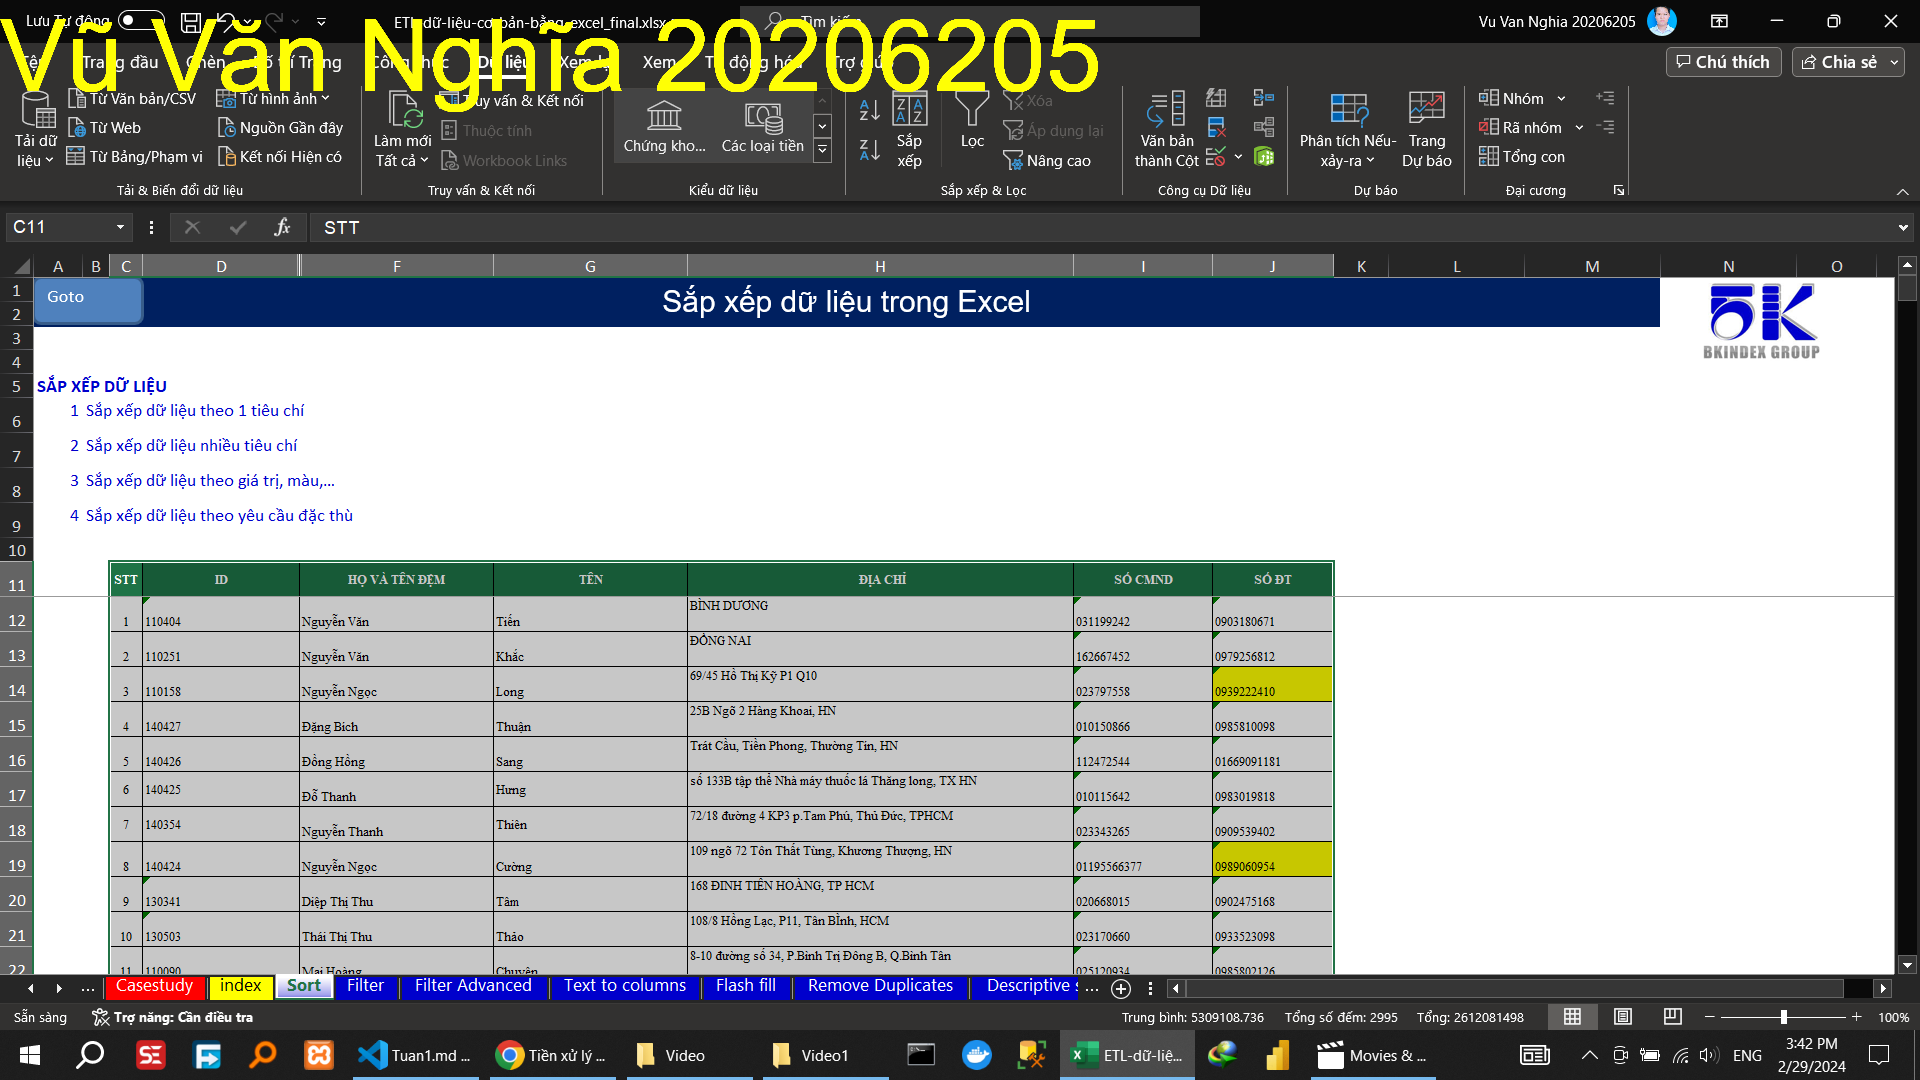
\includegraphics[scale = 0.15]{Video1/HuongDan/1.png}
    \caption{Hướng dẫn sắp xếp dữ liệu theo 1 tiêu chí là số thứ tự}
\end{figure}
% \subparagraph{Hướng dẫn sắp xếp dữ liệu theo nhiều tiêu chí}
\begin{figure}[h]
    \centering
    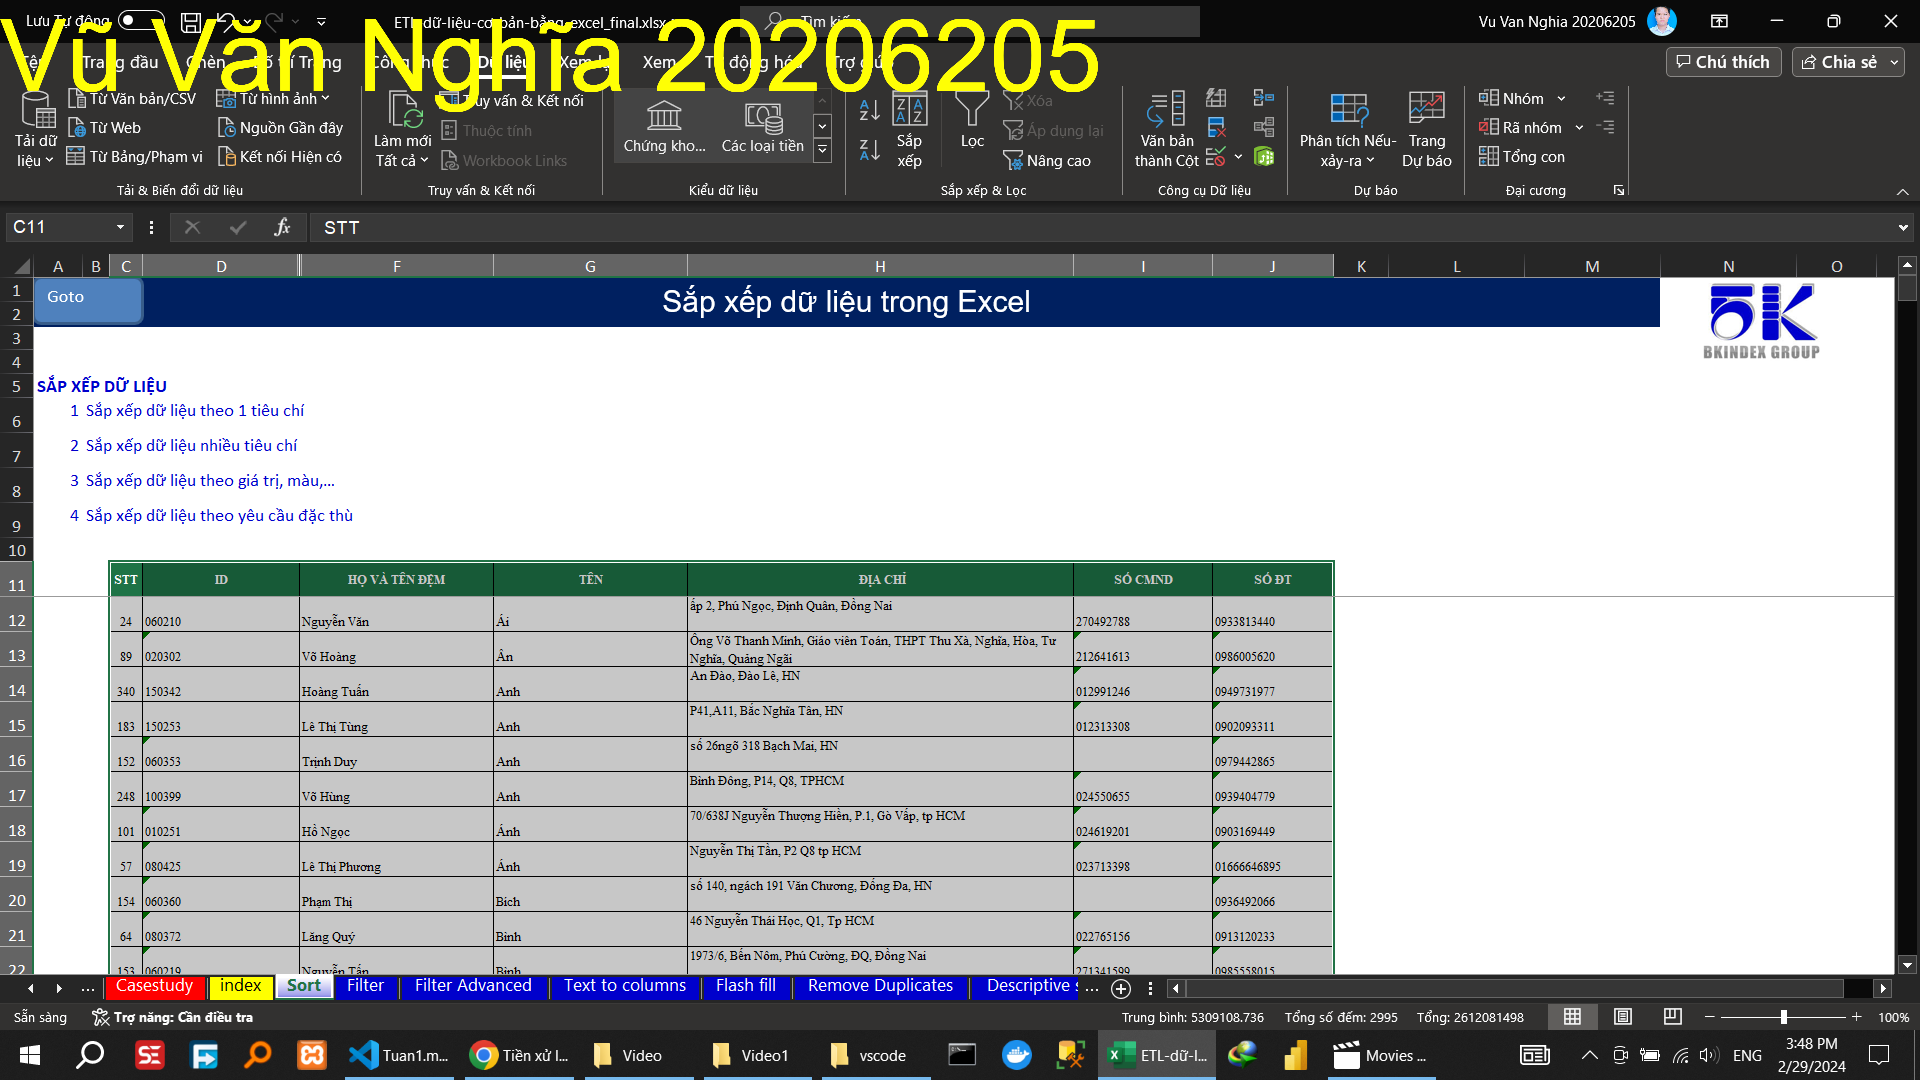
\includegraphics[scale = 0.15]{Video1/HuongDan/2.png}
    \caption{Hướng dẫn sắp xếp dữ liệu theo  nhiều tiêu chí họ và tên đệm}
\end{figure}
% \subparagraph{Hướng dẫn sắp xếp dữ liệu theo giá trị, màu,\dots}
\begin{figure}[h]
    \centering
    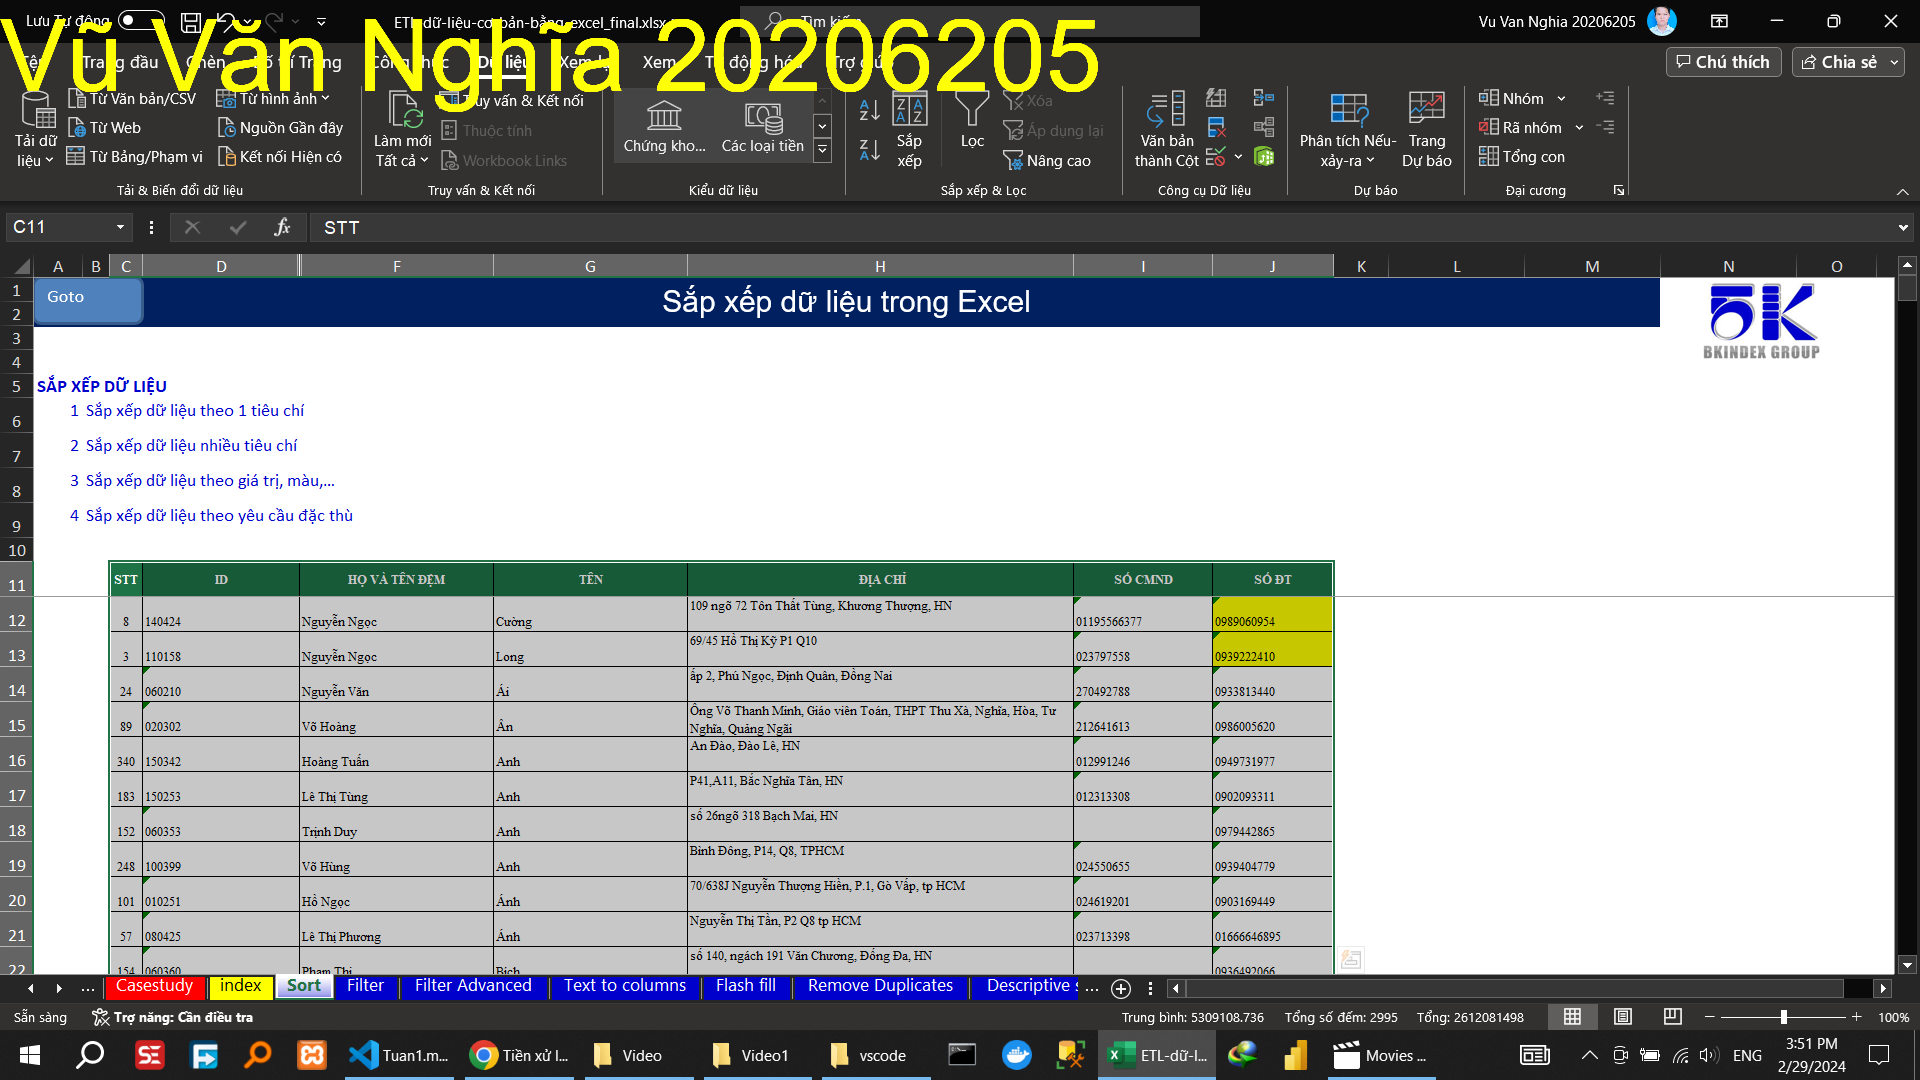
\includegraphics[scale = 0.15]{Video1/HuongDan/3.png}
    \caption{Hướng dẫn sắp xếp dữ liệu theo  giá trị, màu,\dots của số điện thoại}
\end{figure}

% \paragraph{Hướng dẫn lọc dữ liệu}
% \subparagraph{Hướng dẫn lọc dữ liệu theo 1 tiêu chí}
\begin{figure}[h]
    \centering
    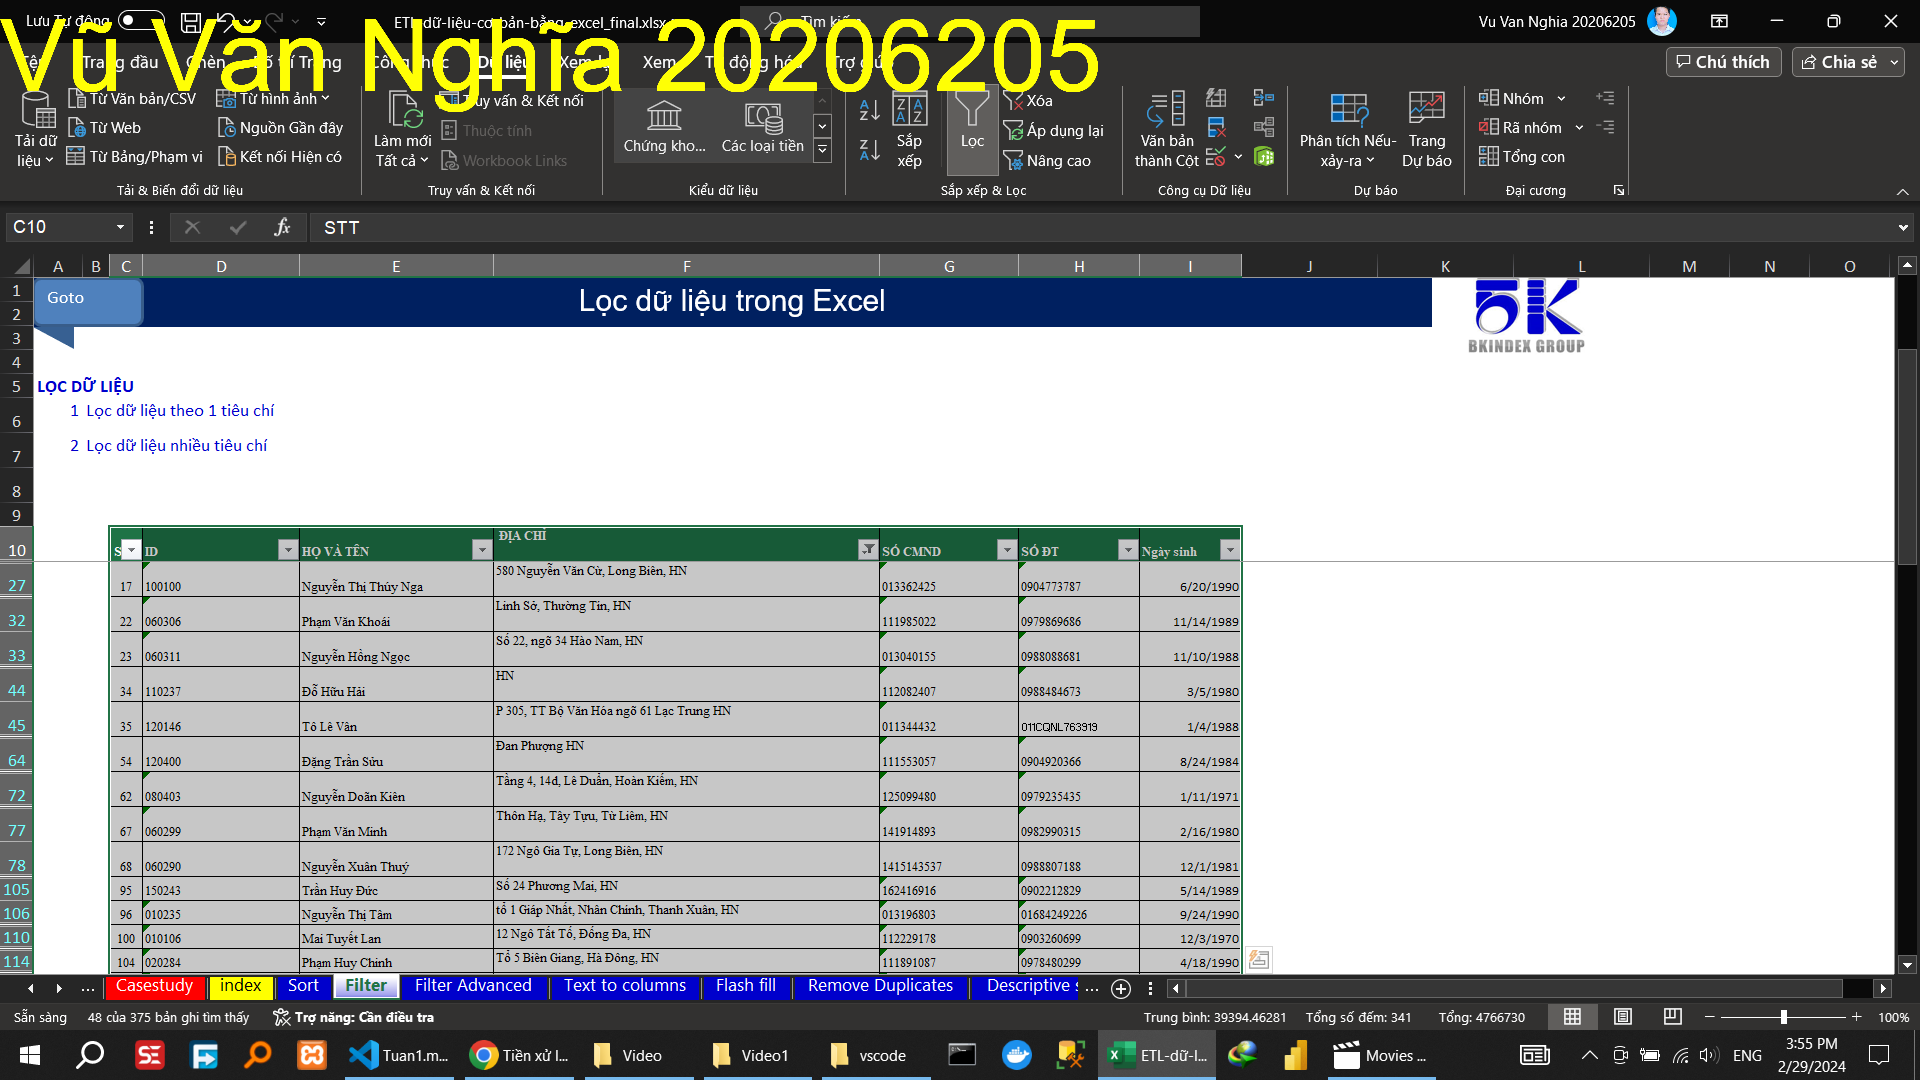
\includegraphics[scale = 0.15]{Video1/HuongDan/4.png}
    \caption{Hướng dẫn lọc dữ liệu theo 1 tiêu chí là địa chỉ HN}
\end{figure}
% \subparagraph{Hướng dẫn lọc dữ liệu theo nhiều tiêu chí}
\begin{figure}[h]
    \centering
    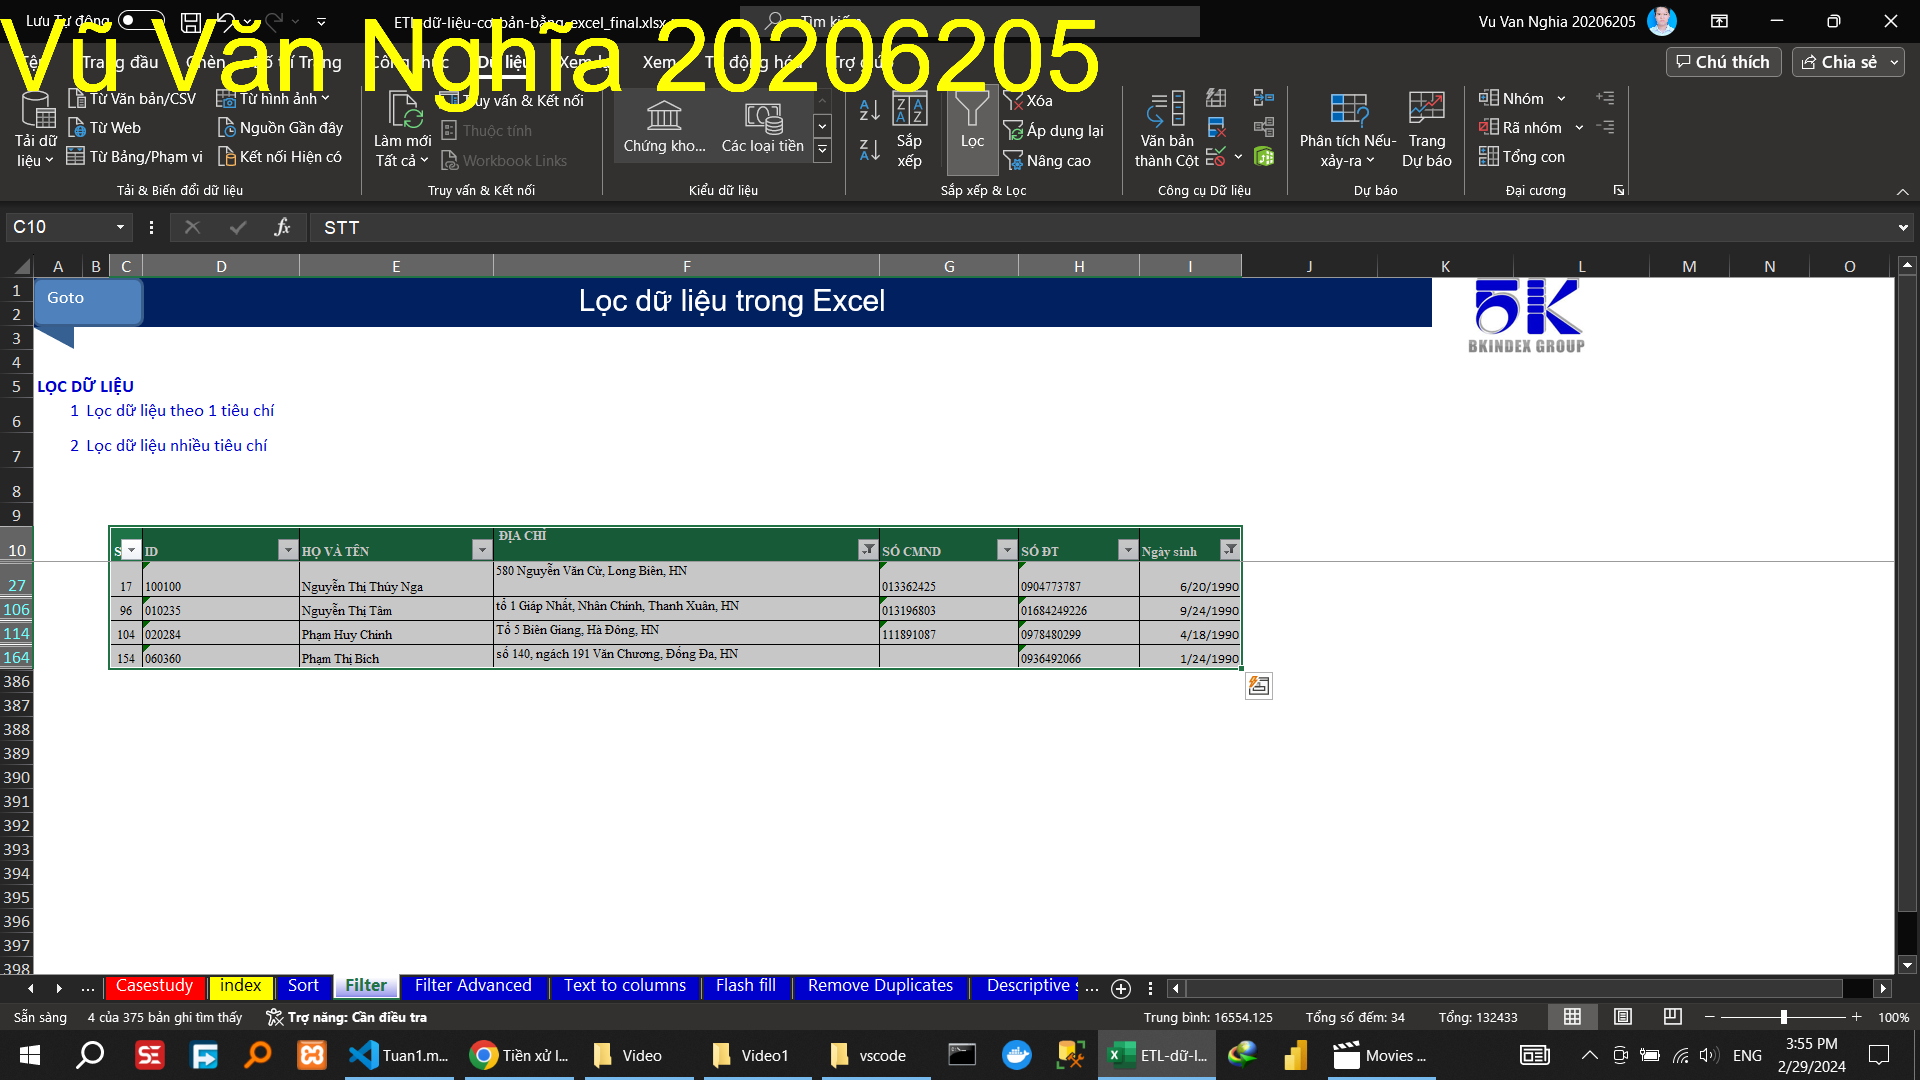
\includegraphics[scale = 0.15]{Video1/HuongDan/5.png}
    \caption{Hướng dẫn lọc dữ liệu theo  nhiều tiêu chí địa chỉ và sinh năm 1990}
\end{figure}




% \paragraph{Hướng dẫn lọc dữ liệu nâng cao}
% \subparagraph{Hướng dẫn lọc dữ liệu nâng cao theo 1 tiêu chí}
\begin{figure}[h]
    \centering
    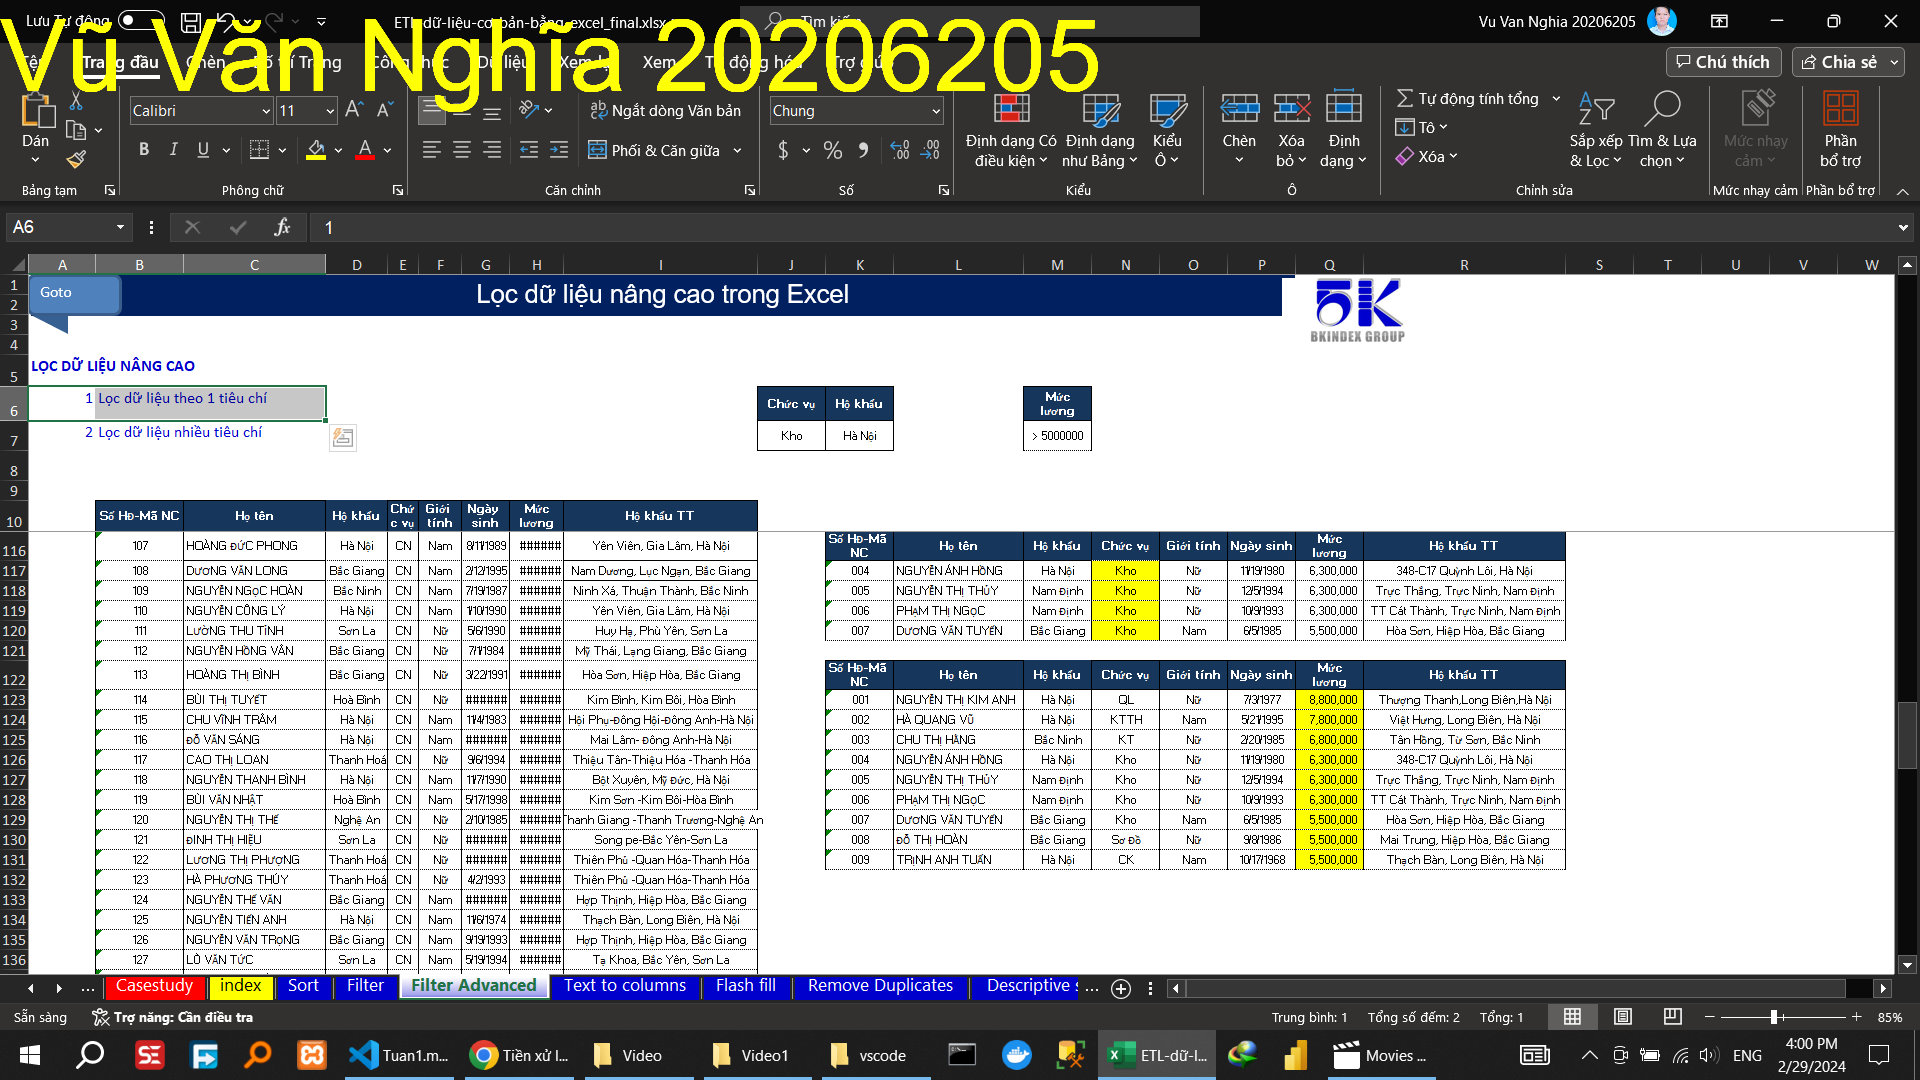
\includegraphics[scale = 0.15]{Video1/HuongDan/6.png}
    \caption{Hướng dẫn lọc dữ liệu nâng cao theo 1 tiêu chí là chức vụ hoặc mức lương}
\end{figure}
% \subparagraph{Hướng dẫn lọc dữ liệu nâng cao theo nhiều tiêu chí}
\begin{figure}[h]
    \centering
    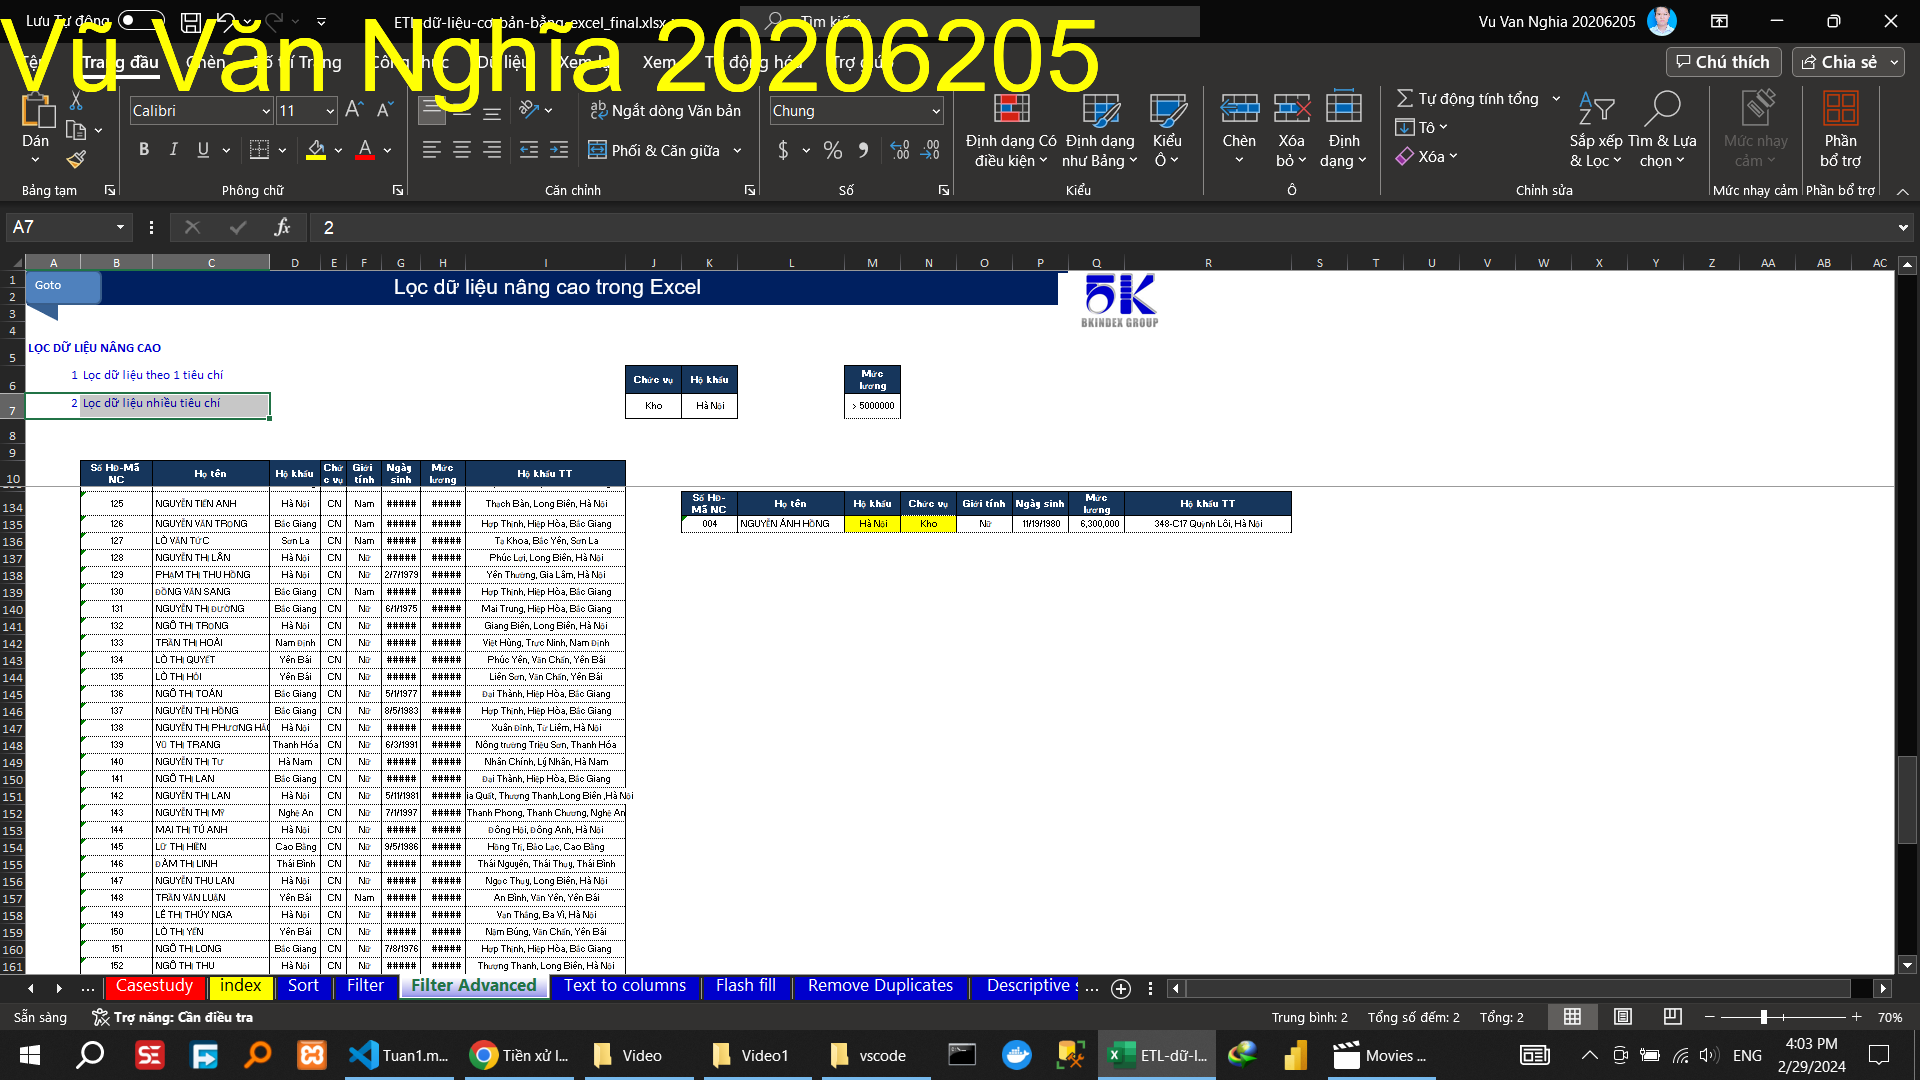
\includegraphics[scale = 0.15]{Video1/HuongDan/7.png}
    \caption{Hướng dẫn lọc dữ liệu nâng cao theo  nhiều tiêu chí  chức vụ và hộ khẩu}
\end{figure}



% \paragraph{Hướng dẫn tách cột văn bản thành nhiều cột}
% \subparagraph{Hướng dẫn  tách ngày tháng}
\begin{figure}[h]
    \centering
    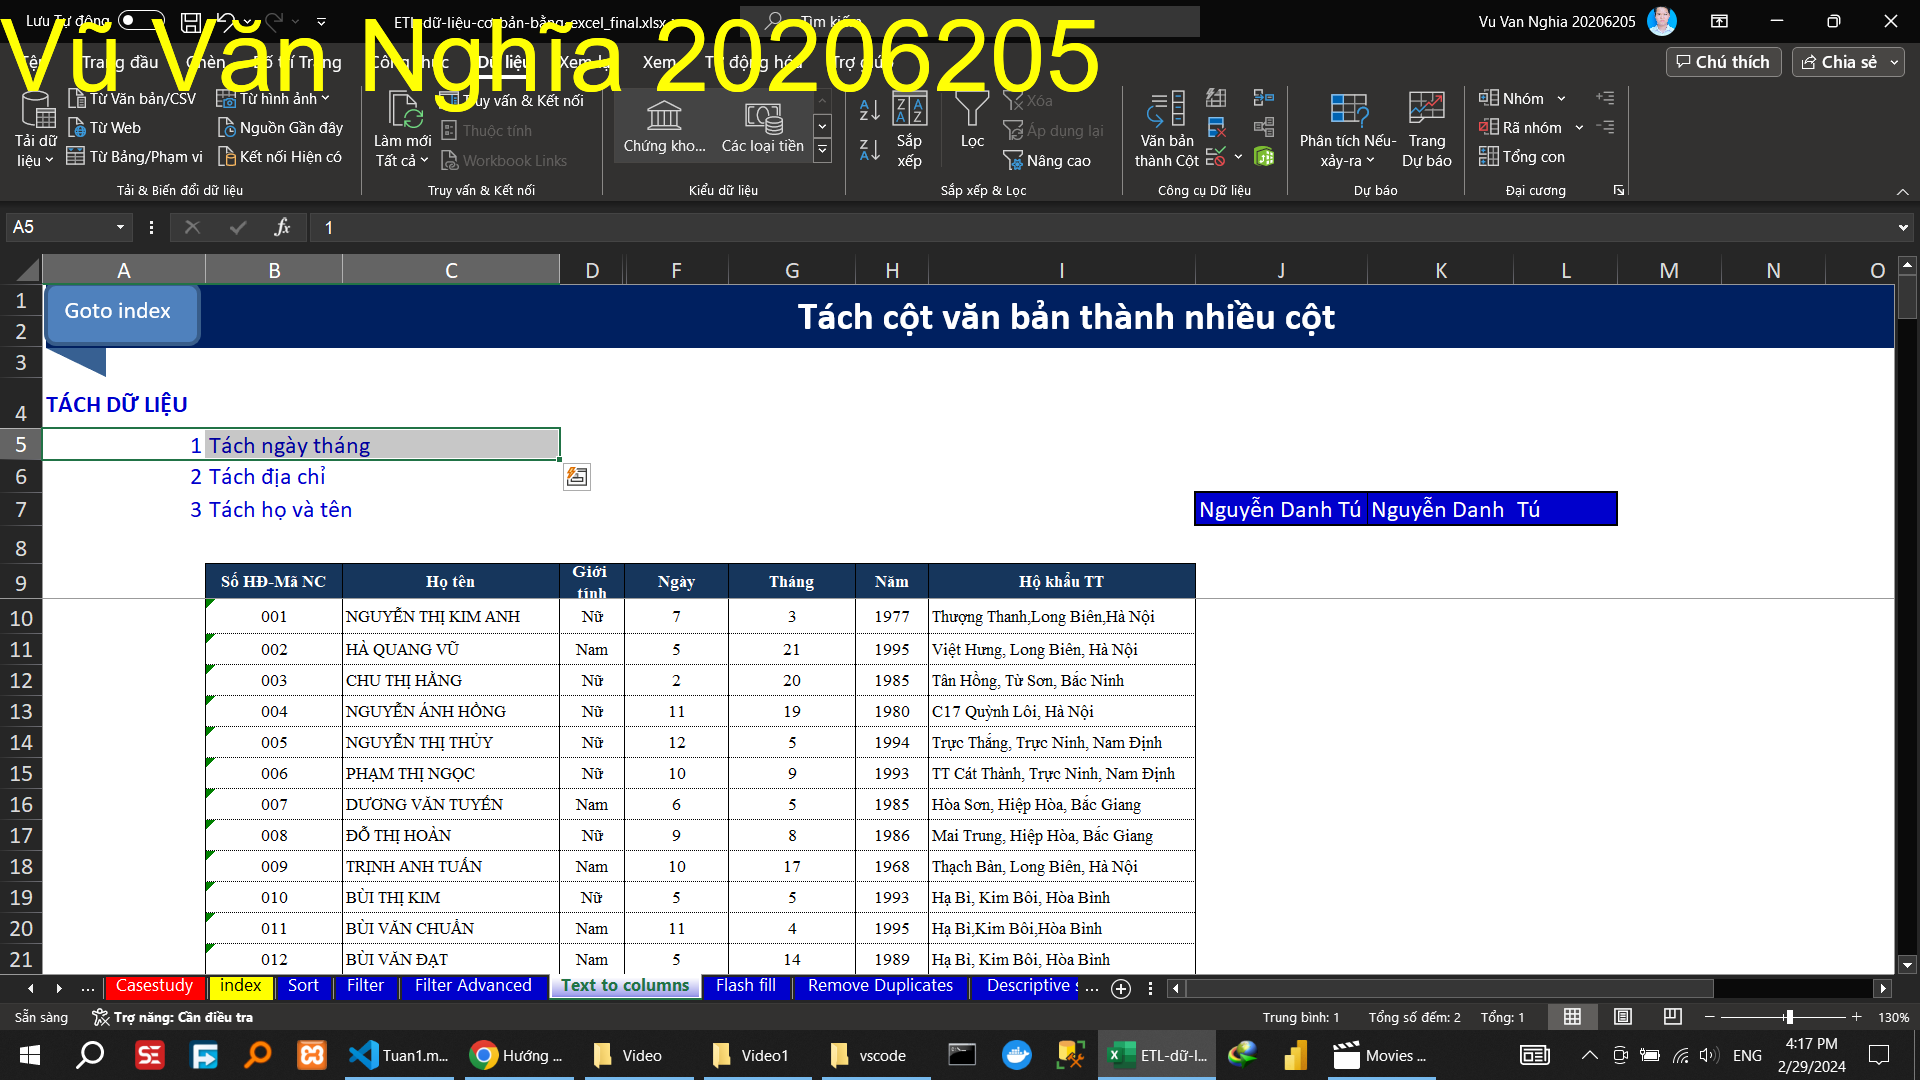
\includegraphics[scale = 0.15]{Video1/HuongDan/8.png}
    \caption{Hướng dẫn  tách ngày tháng}
\end{figure} 
% \subparagraph{Hướng dẫn  tách  địa chỉ}
\begin{figure}[h]
    \centering
    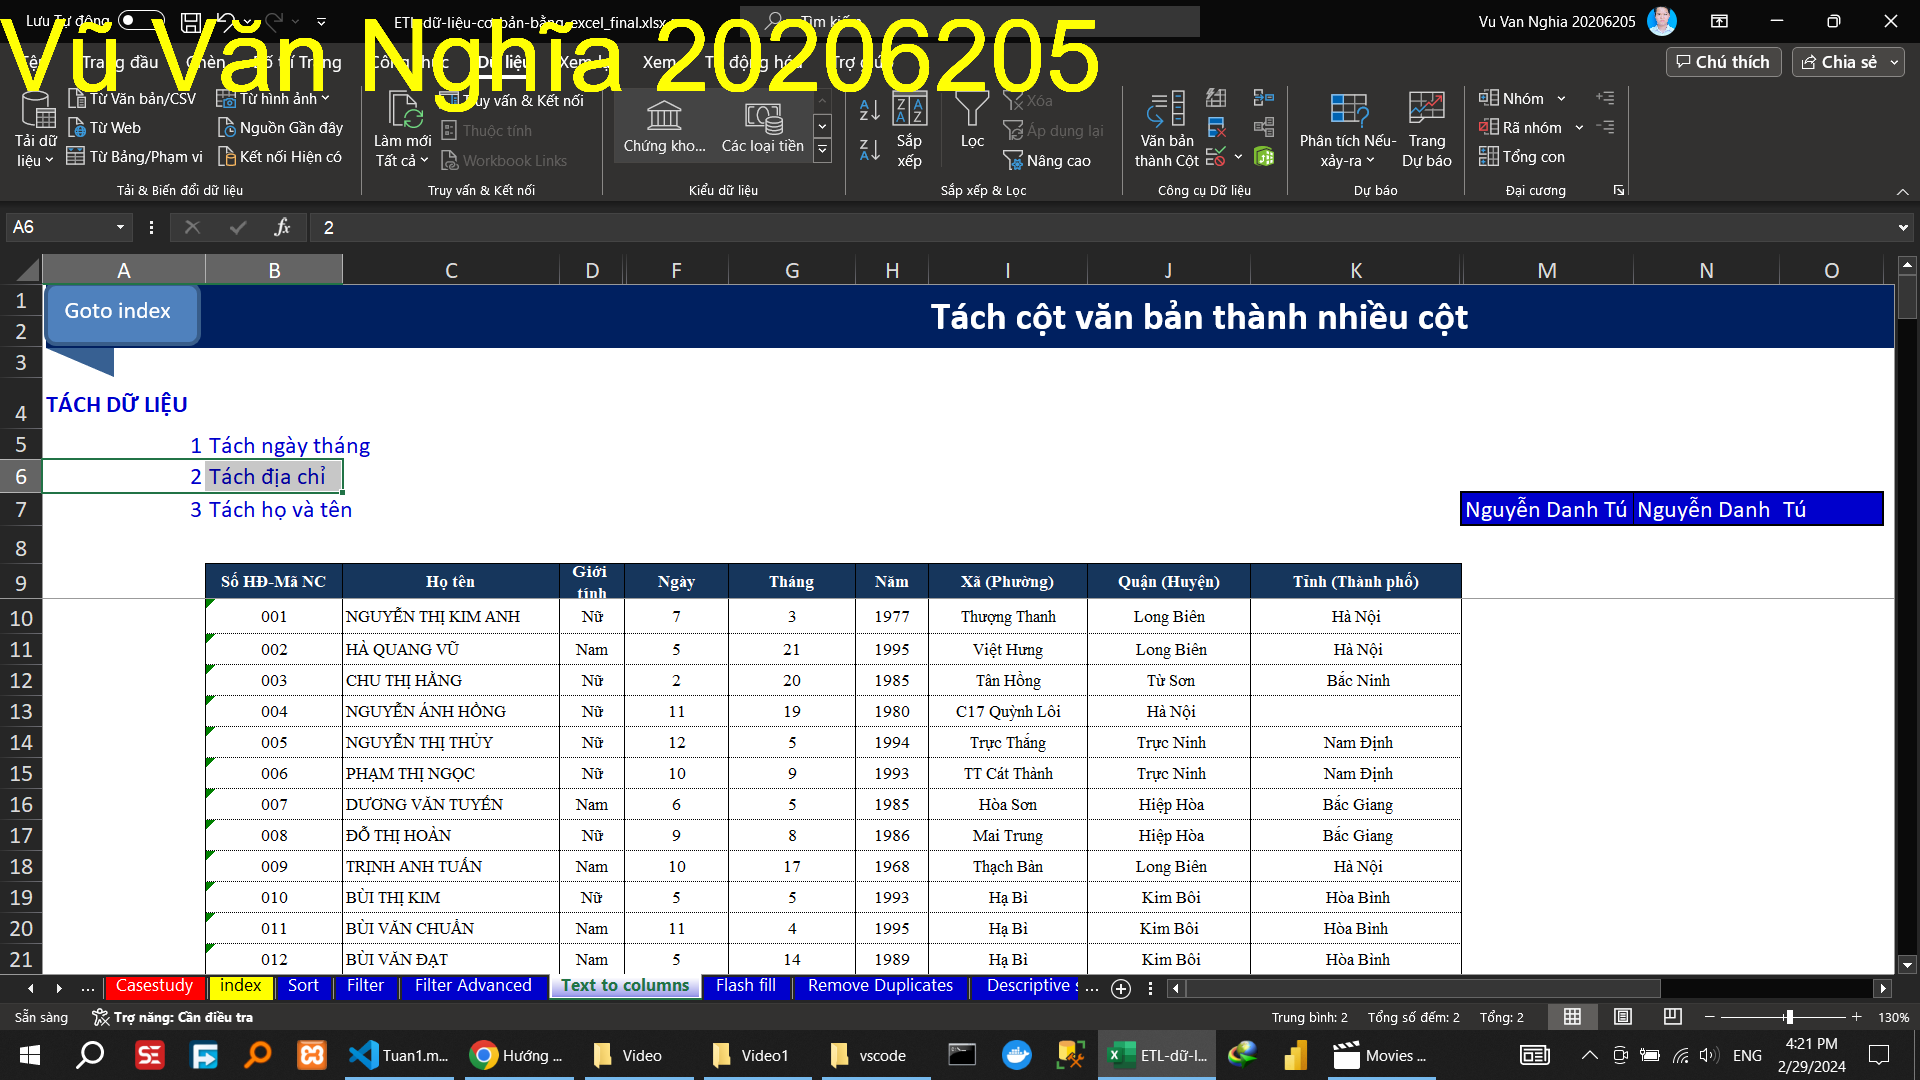
\includegraphics[scale = 0.15]{Video1/HuongDan/9.png}
    \caption{Hướng dẫn  tách  địa chỉ}
\end{figure} 
% \subparagraph{Hướng dẫn  tách  họ và tên}
\begin{figure}[h]
    \centering
    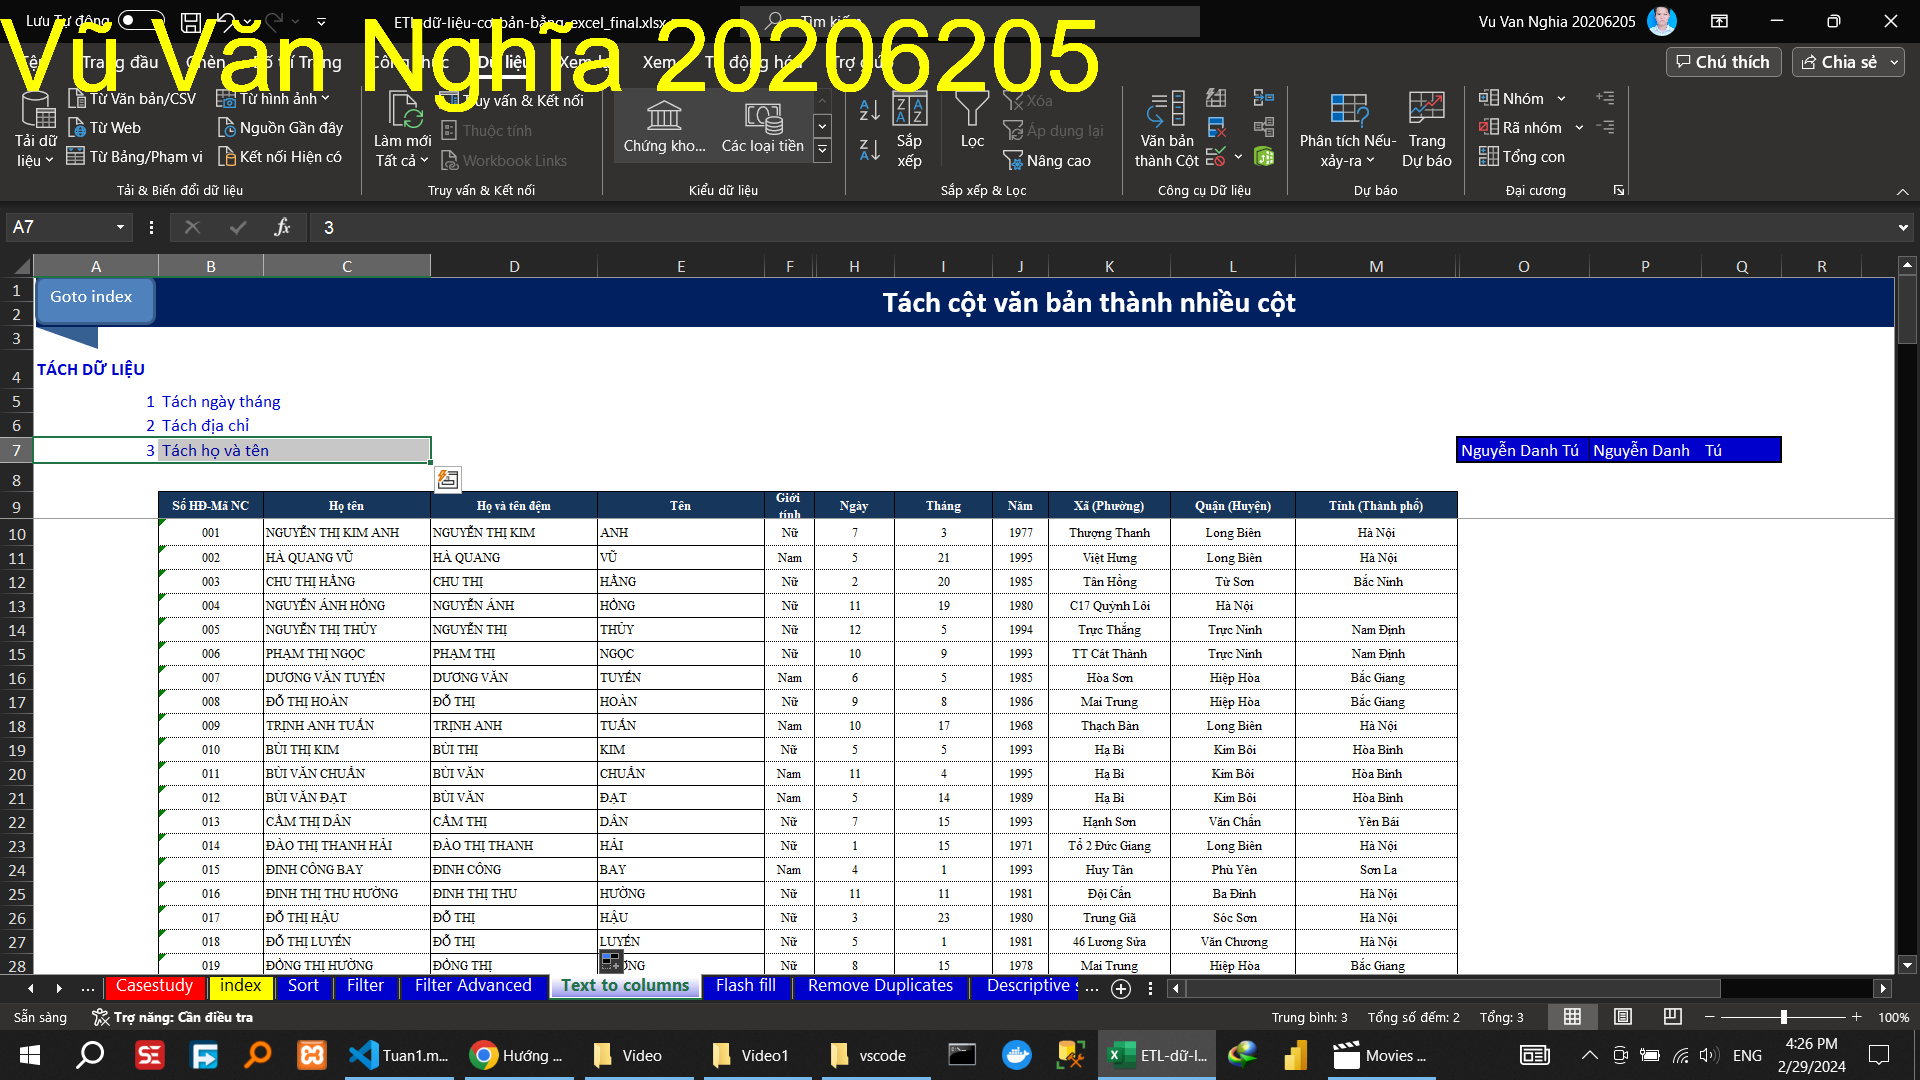
\includegraphics[scale = 0.15]{Video1/HuongDan/10.png}
    \caption{Hướng dẫn  tách  họ và tên}
\end{figure} 




% \paragraph{Hướng dẫn điền dữ liệu tự động}
% \subparagraph{Hướng dẫn điền dữ liệu tự động}
\begin{figure}[h]
    \centering
    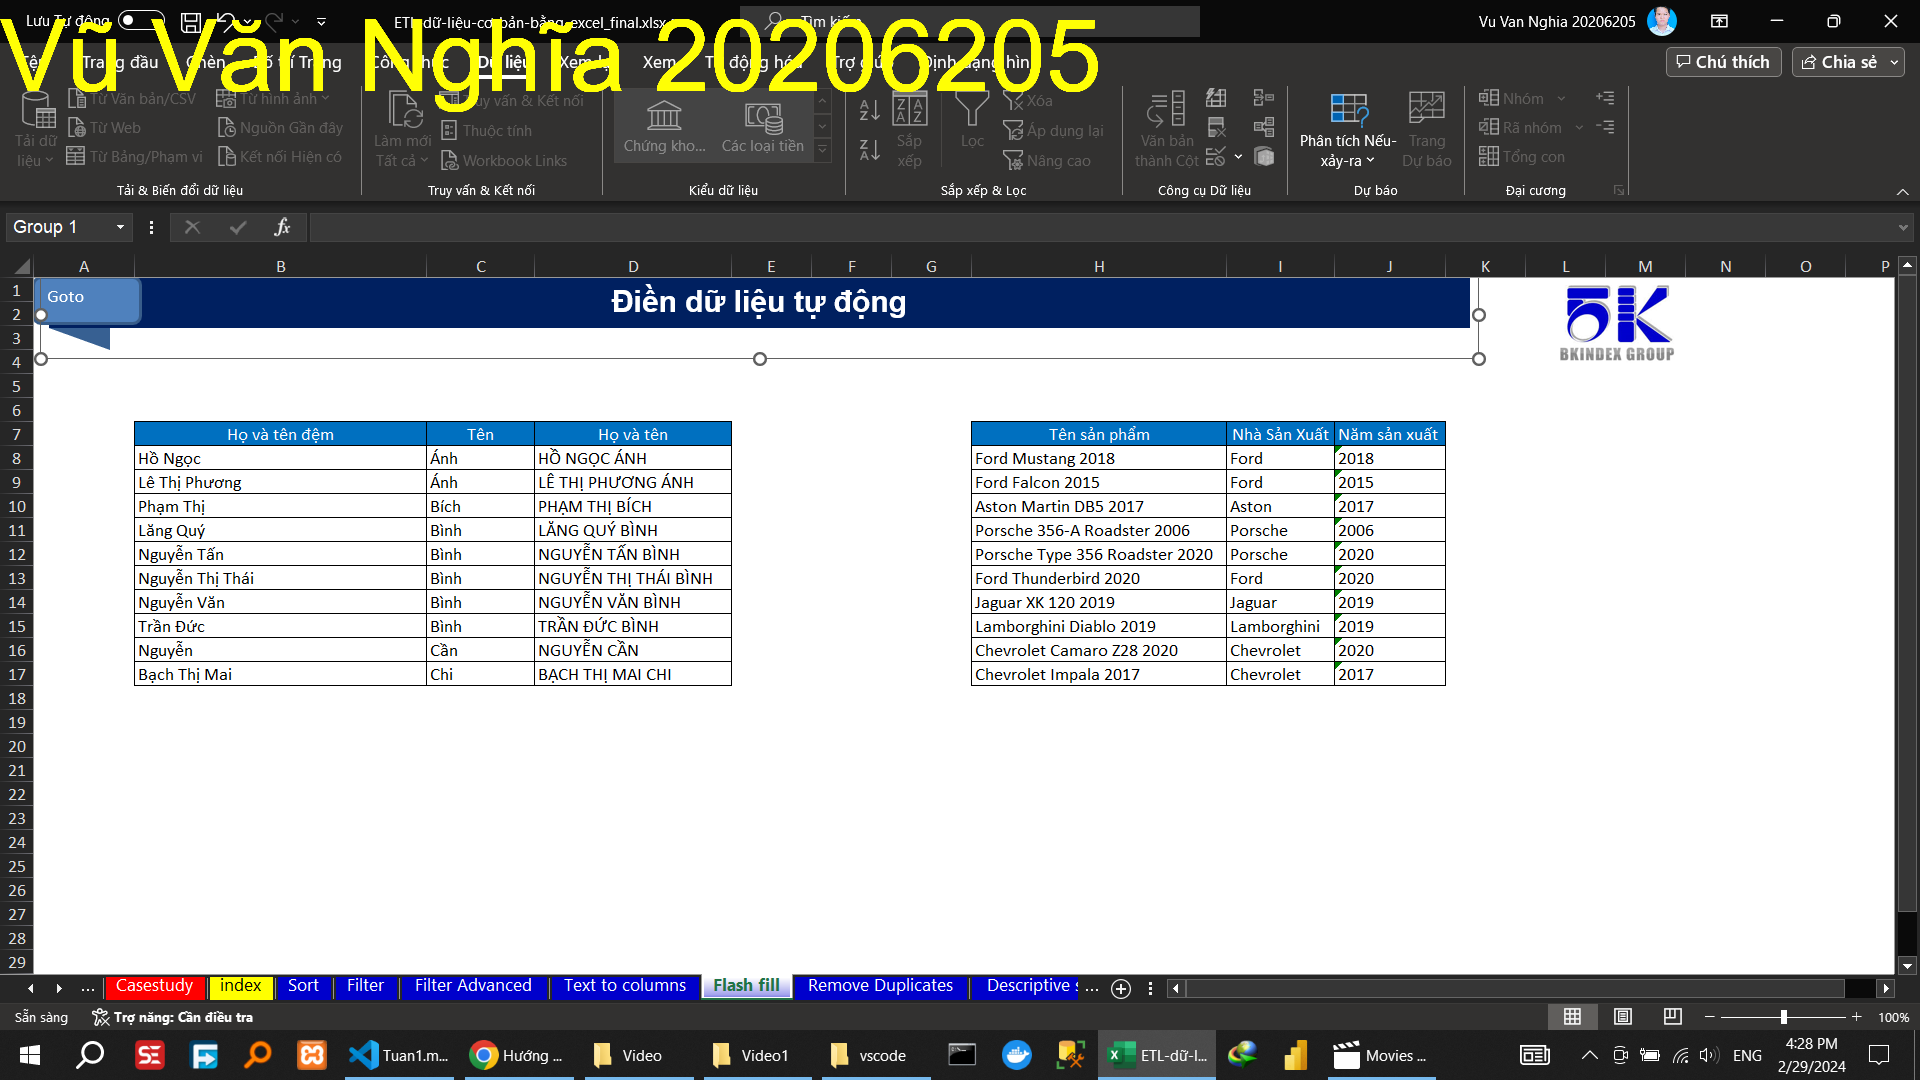
\includegraphics[scale = 0.15]{Video1/HuongDan/11.png}
    \caption{Hướng dẫn điền dữ liệu tự động}
\end{figure}

% \paragraph{Hướng dẫn xóa dữ liệu bị trùng}
% \subparagraph{Hướng dẫn xóa dữ liệu bị trùng}
\begin{figure}[h]
    \centering
    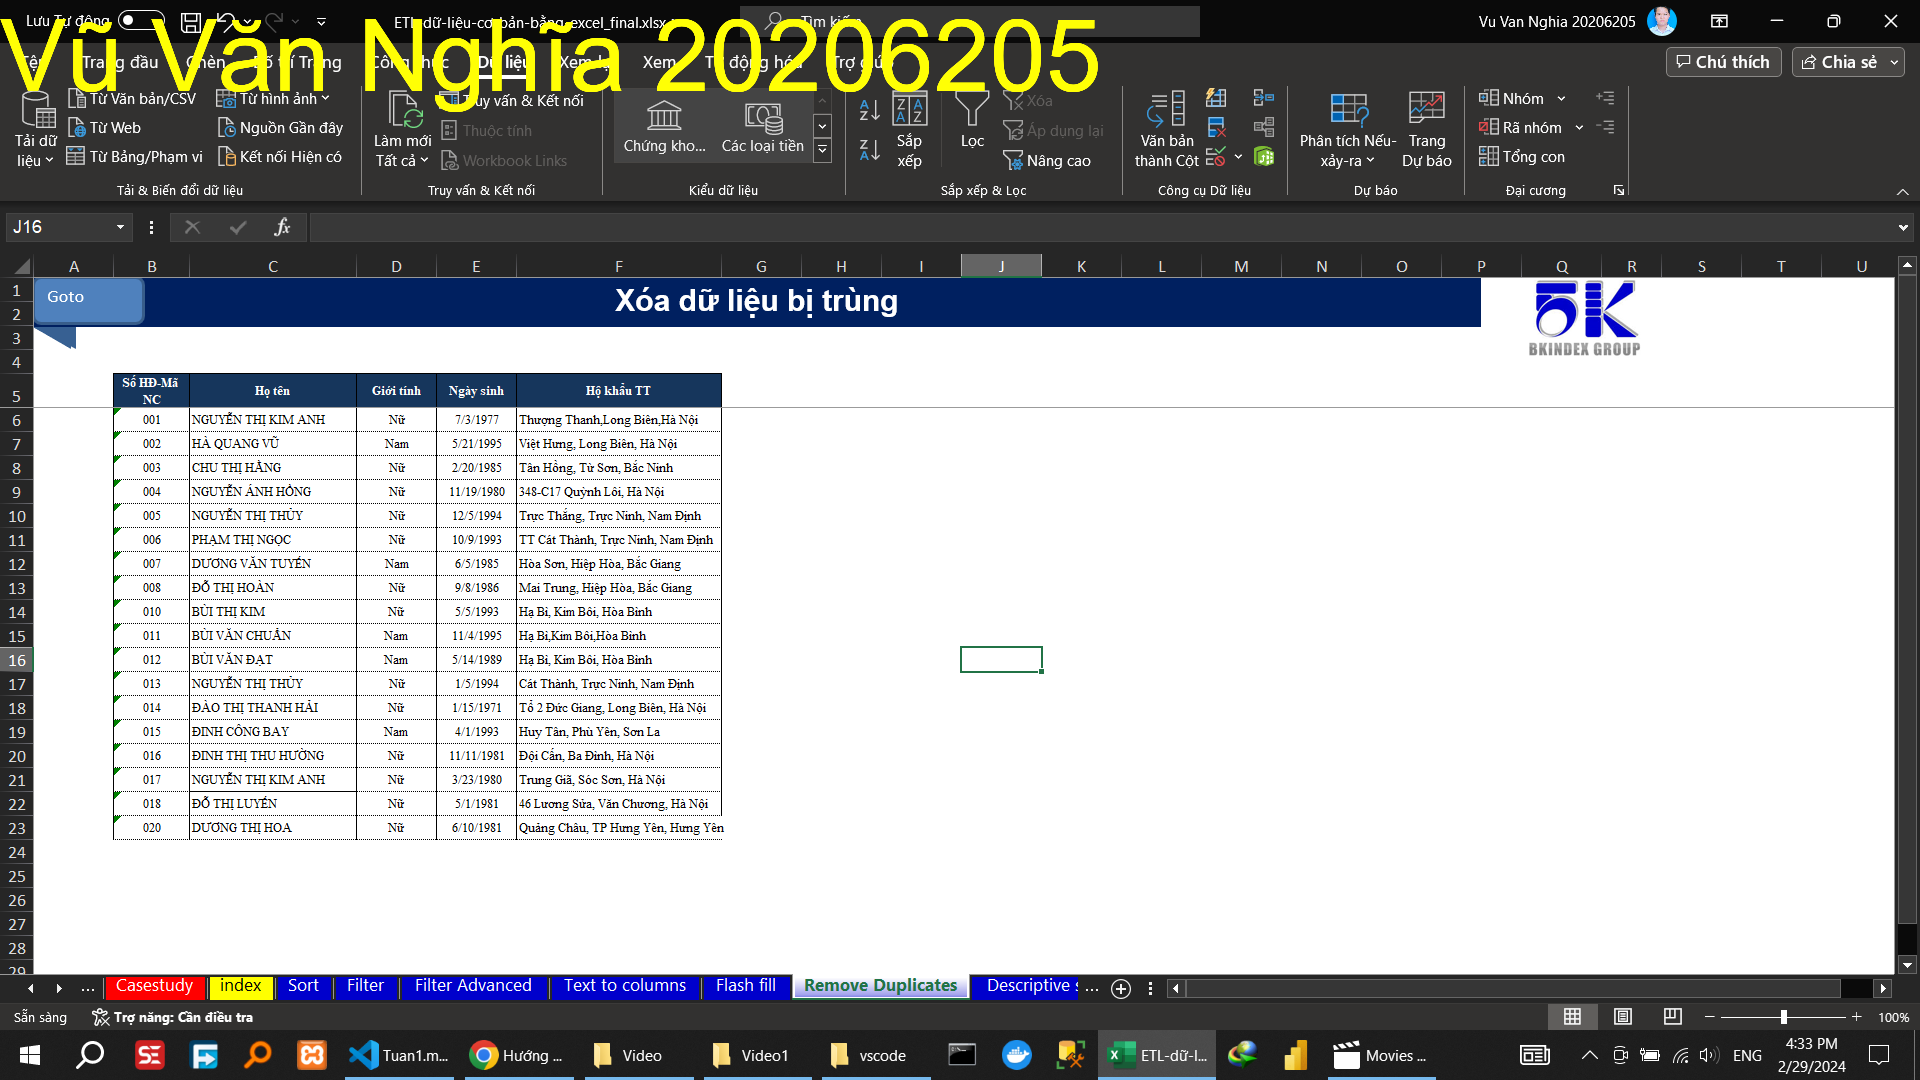
\includegraphics[scale = 0.15]{Video1/HuongDan/12.png}
    \caption{Hướng dẫn xóa dữ liệu bị trùng}
\end{figure}

% \paragraph{Hướng dẫn thống kê mô tả}
% \subparagraph{Hướng dẫn thống kê mô tả}
\begin{figure}[h]
    \centering
    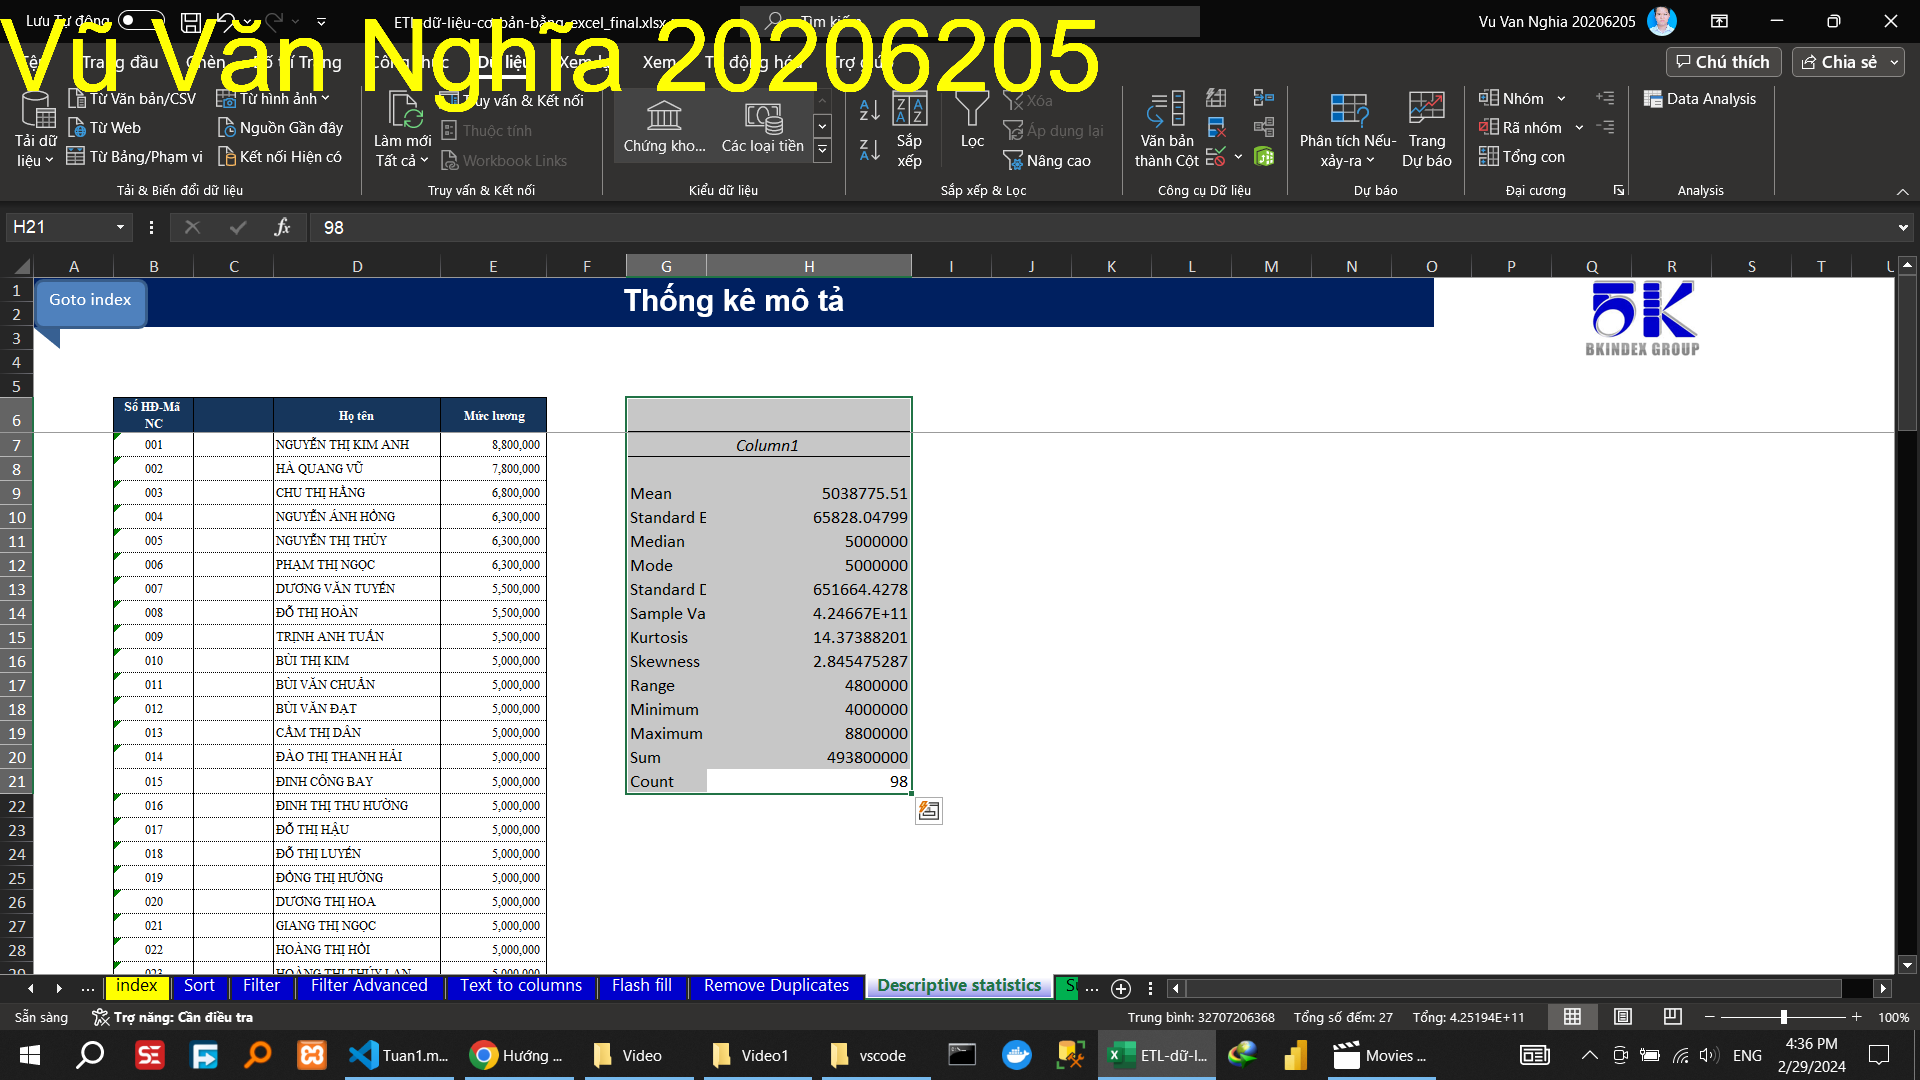
\includegraphics[scale = 0.15]{Video1/HuongDan/13.png}
    \caption{Hướng dẫn thống kê mô tả}
\end{figure}



\subsubsection{Thực hành}

% \paragraph{Thực hành bỏ vùng trộn (merge)}
% \subparagraph{Thực hành bỏ vùng trộn (merge)}
\begin{figure}[h]
    \centering
    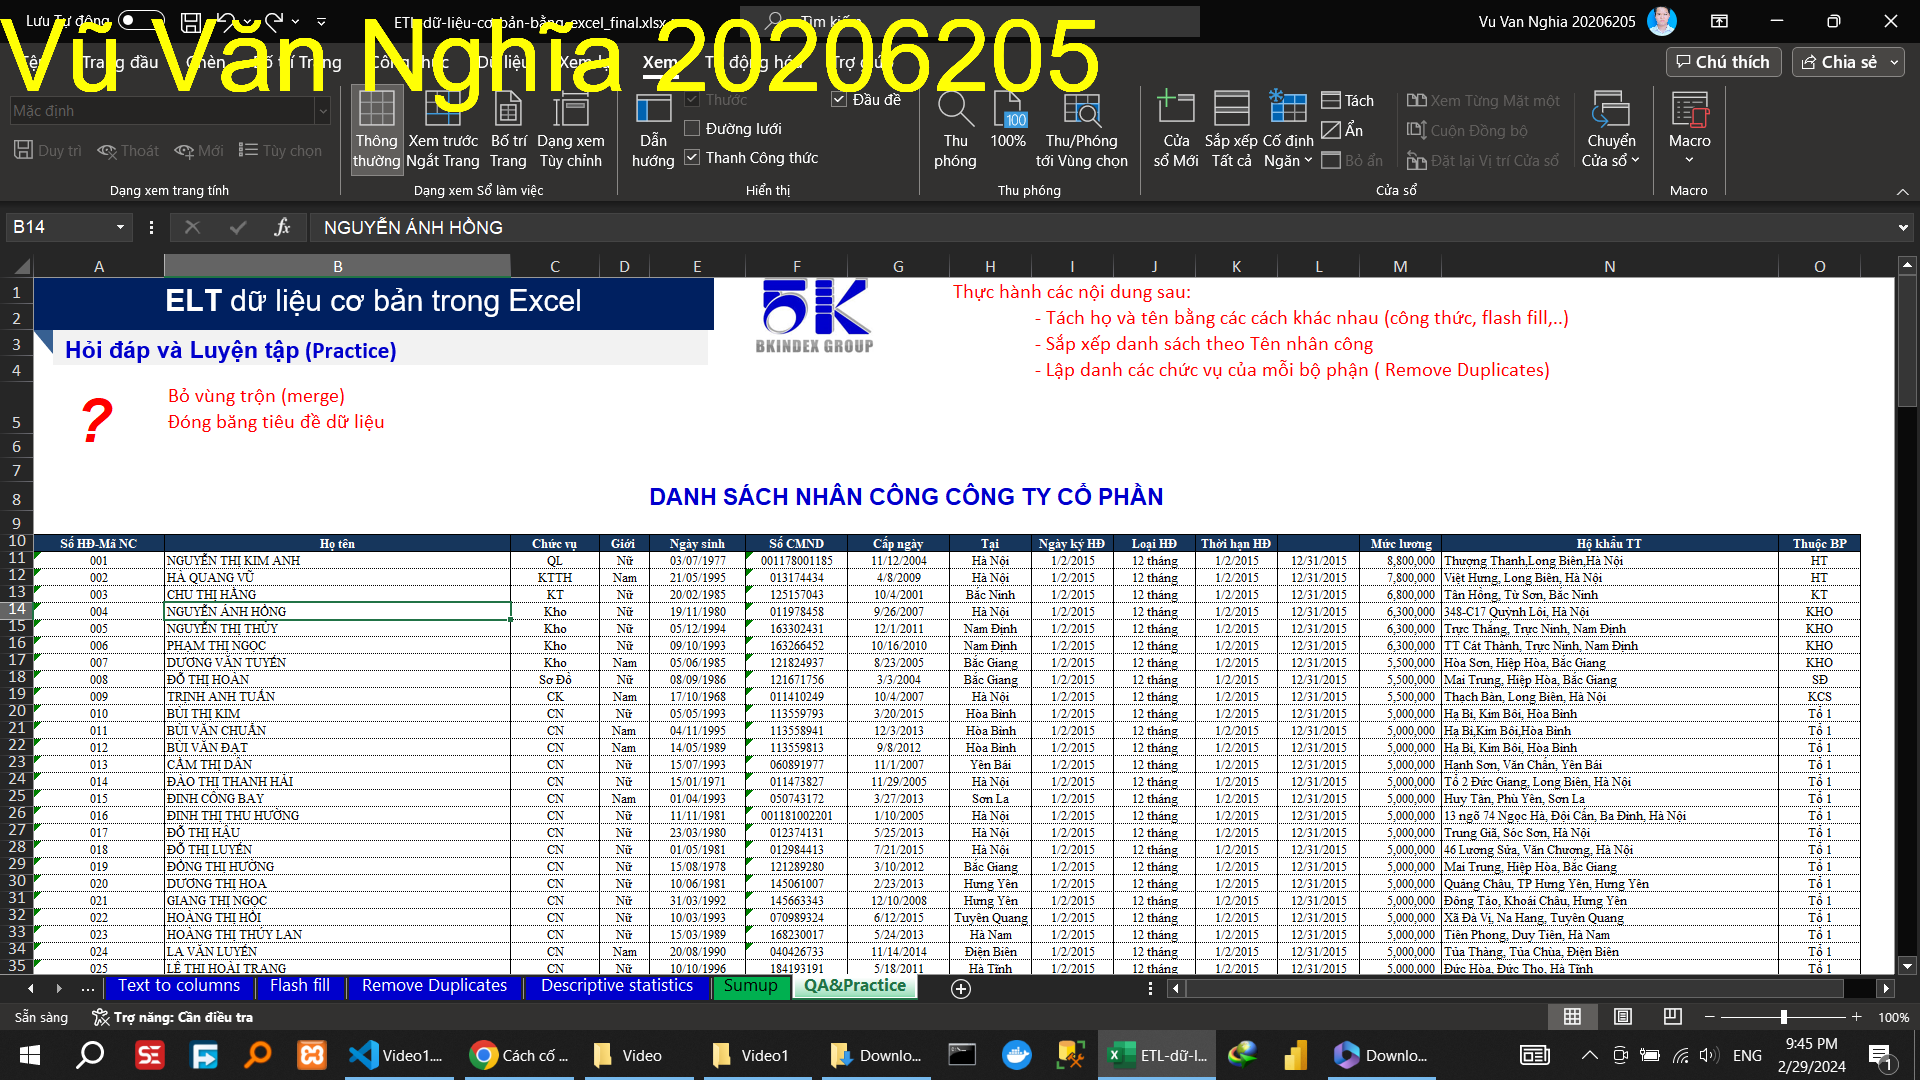
\includegraphics[scale = 0.15]{Video1/ThucHanh/1.png}
\caption{Thực hành bỏ vùng trộn (merge)}
\end{figure}

% \paragraph{Thực hành  đóng băng tiêu đề dữ liệu}
% \subparagraph{Thực hành  đóng băng tiêu đề dữ liệu}
\begin{figure}[h]
    \centering
    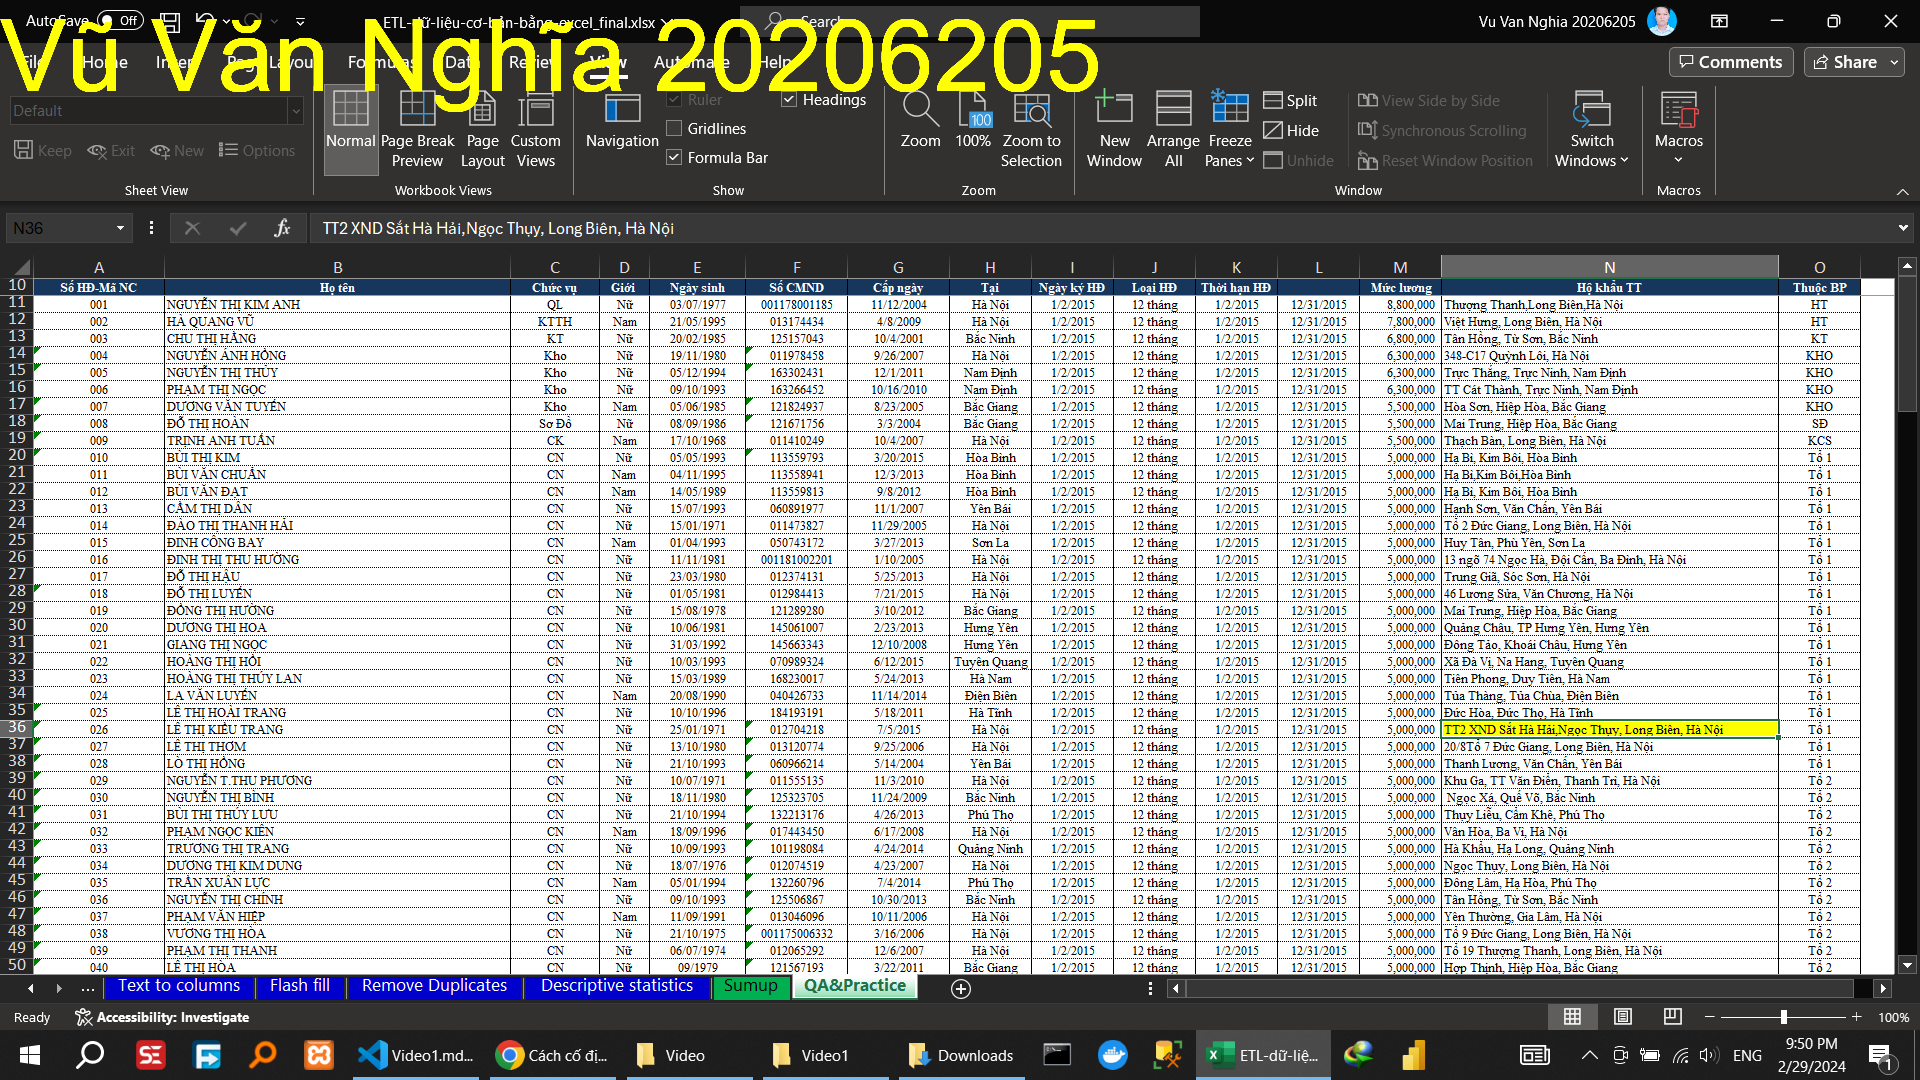
\includegraphics[scale = 0.15]{Video1/ThucHanh/2.png}
\caption{Thực hành  đóng băng tiêu đề dữ liệu}
\end{figure}

% \paragraph{Thực hành tách họ và tên bằng công thức}
% \subparagraph{Thực hành tách họ và tên bằng công thức}
\begin{figure}[h]
    \centering
    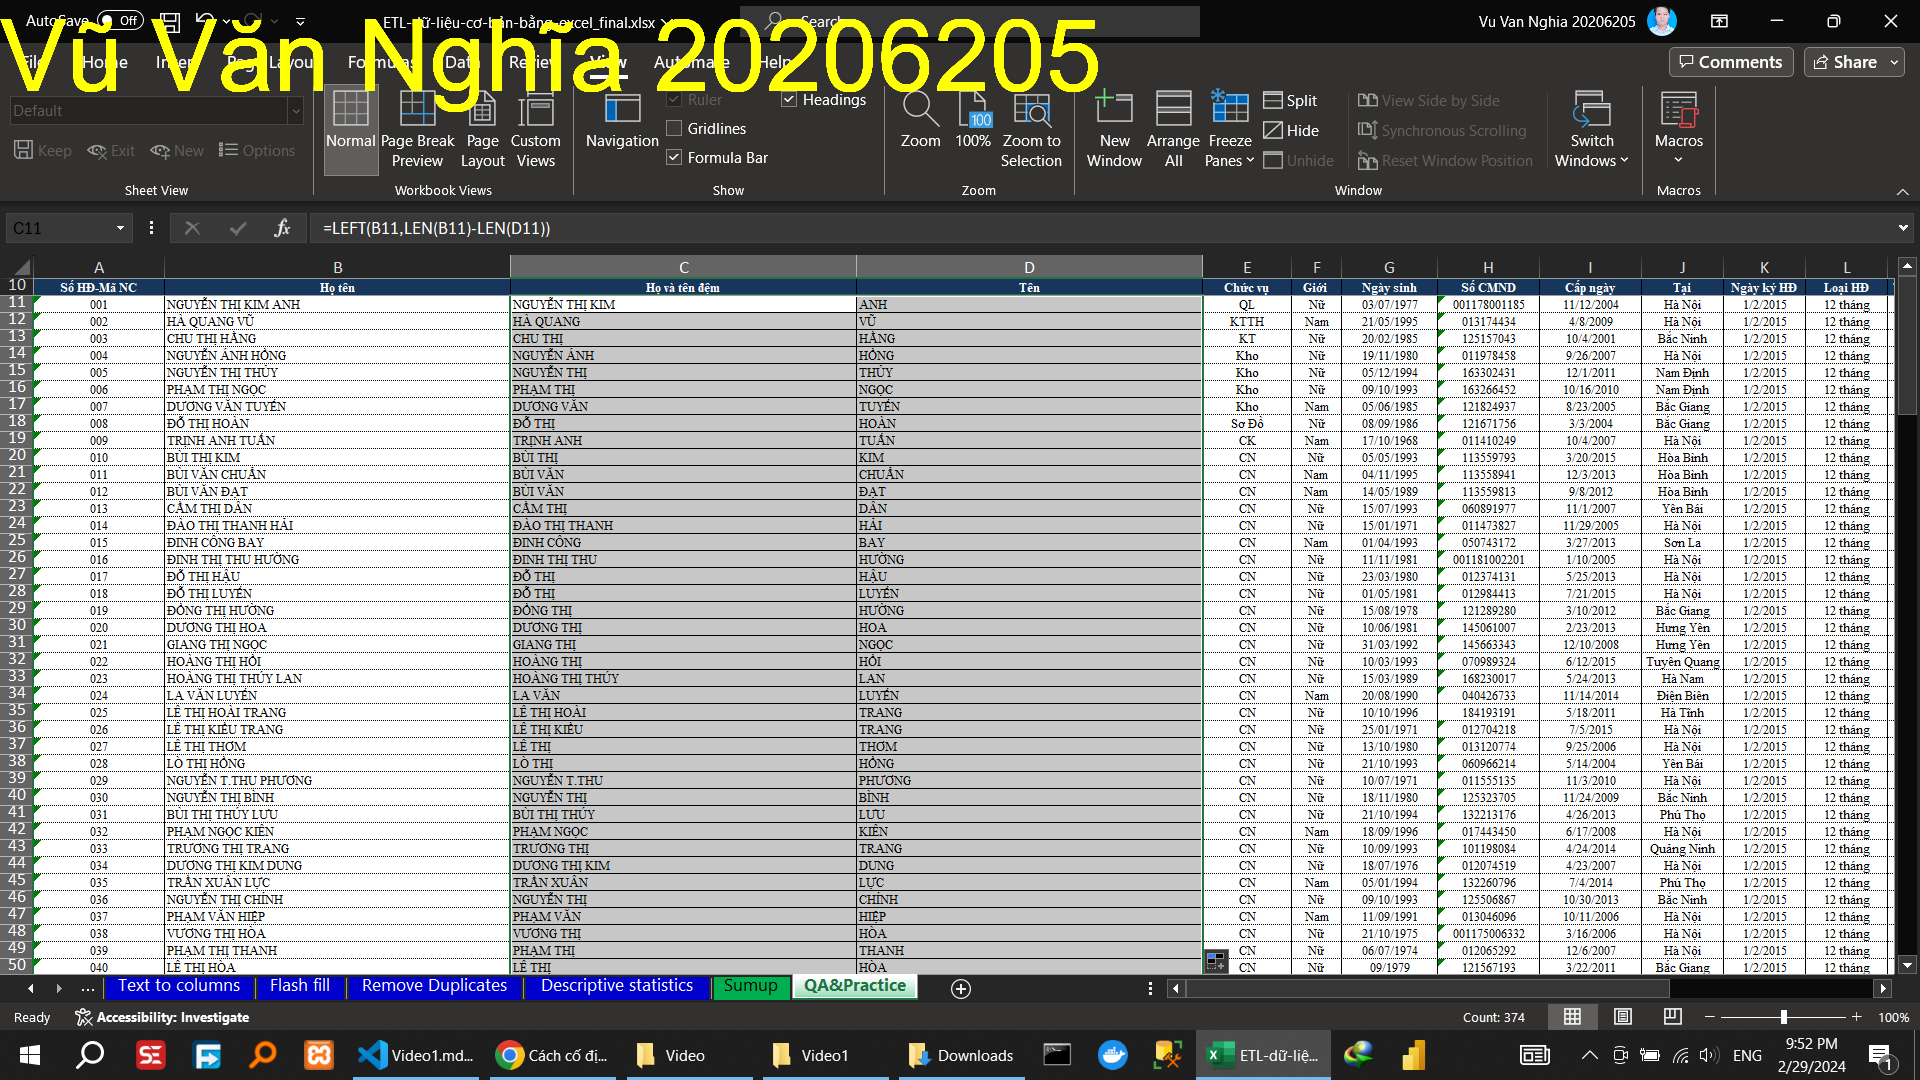
\includegraphics[scale = 0.15]{Video1/ThucHanh/3.png}
\caption{Thực hành tách họ và tên bằng công thức}
\end{figure}


% \paragraph{Thực hành   tách họ và tên bằng flash fill}
% \subparagraph{Thực hành   tách họ và tên bằng flash fill}
\begin{figure}[h]
    \centering
    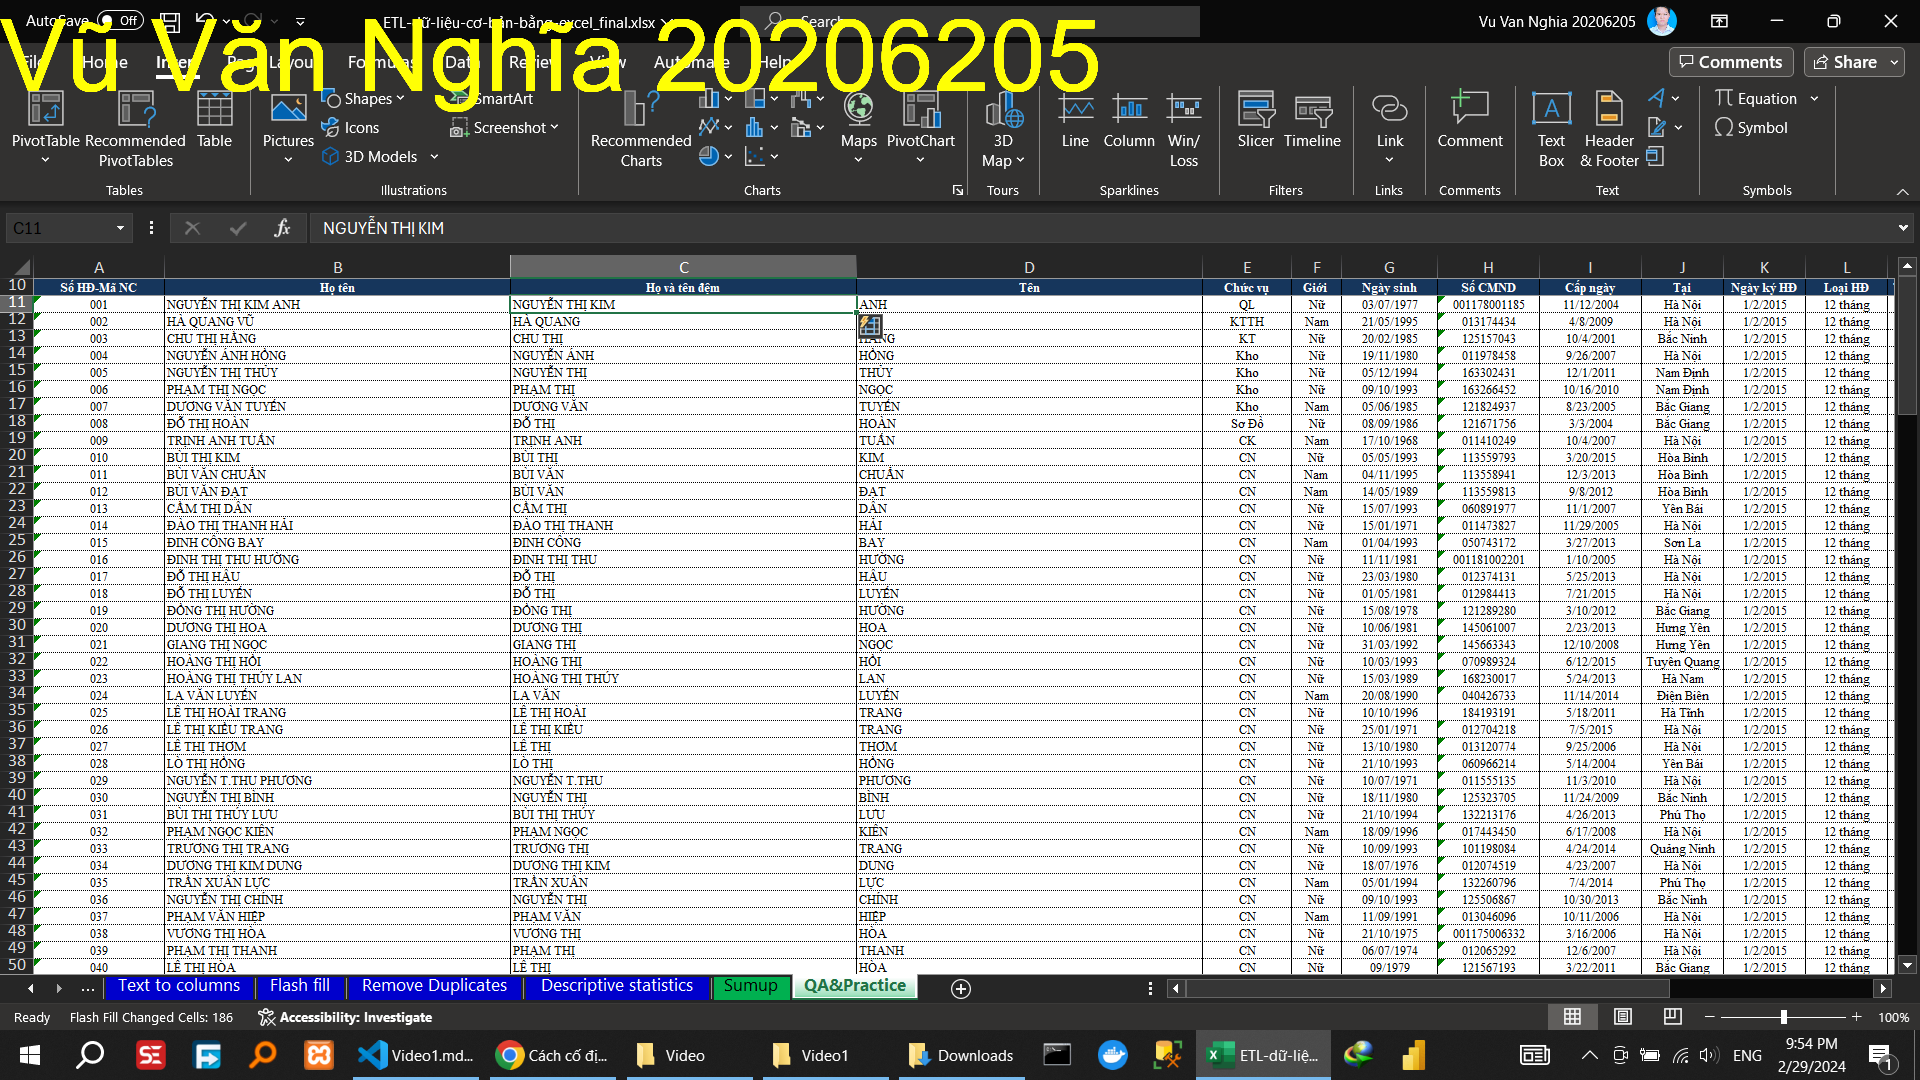
\includegraphics[scale = 0.15]{Video1/ThucHanh/4.png}
\caption{Thực hành   tách họ và tên bằng flash fill}
\end{figure}



% \paragraph{Thực hành  sắp xếp danh sách theo tên nhân công}
% \subparagraph{Thực hành  sắp xếp danh sách theo tên nhân công}
\begin{figure}[h]
    \centering
    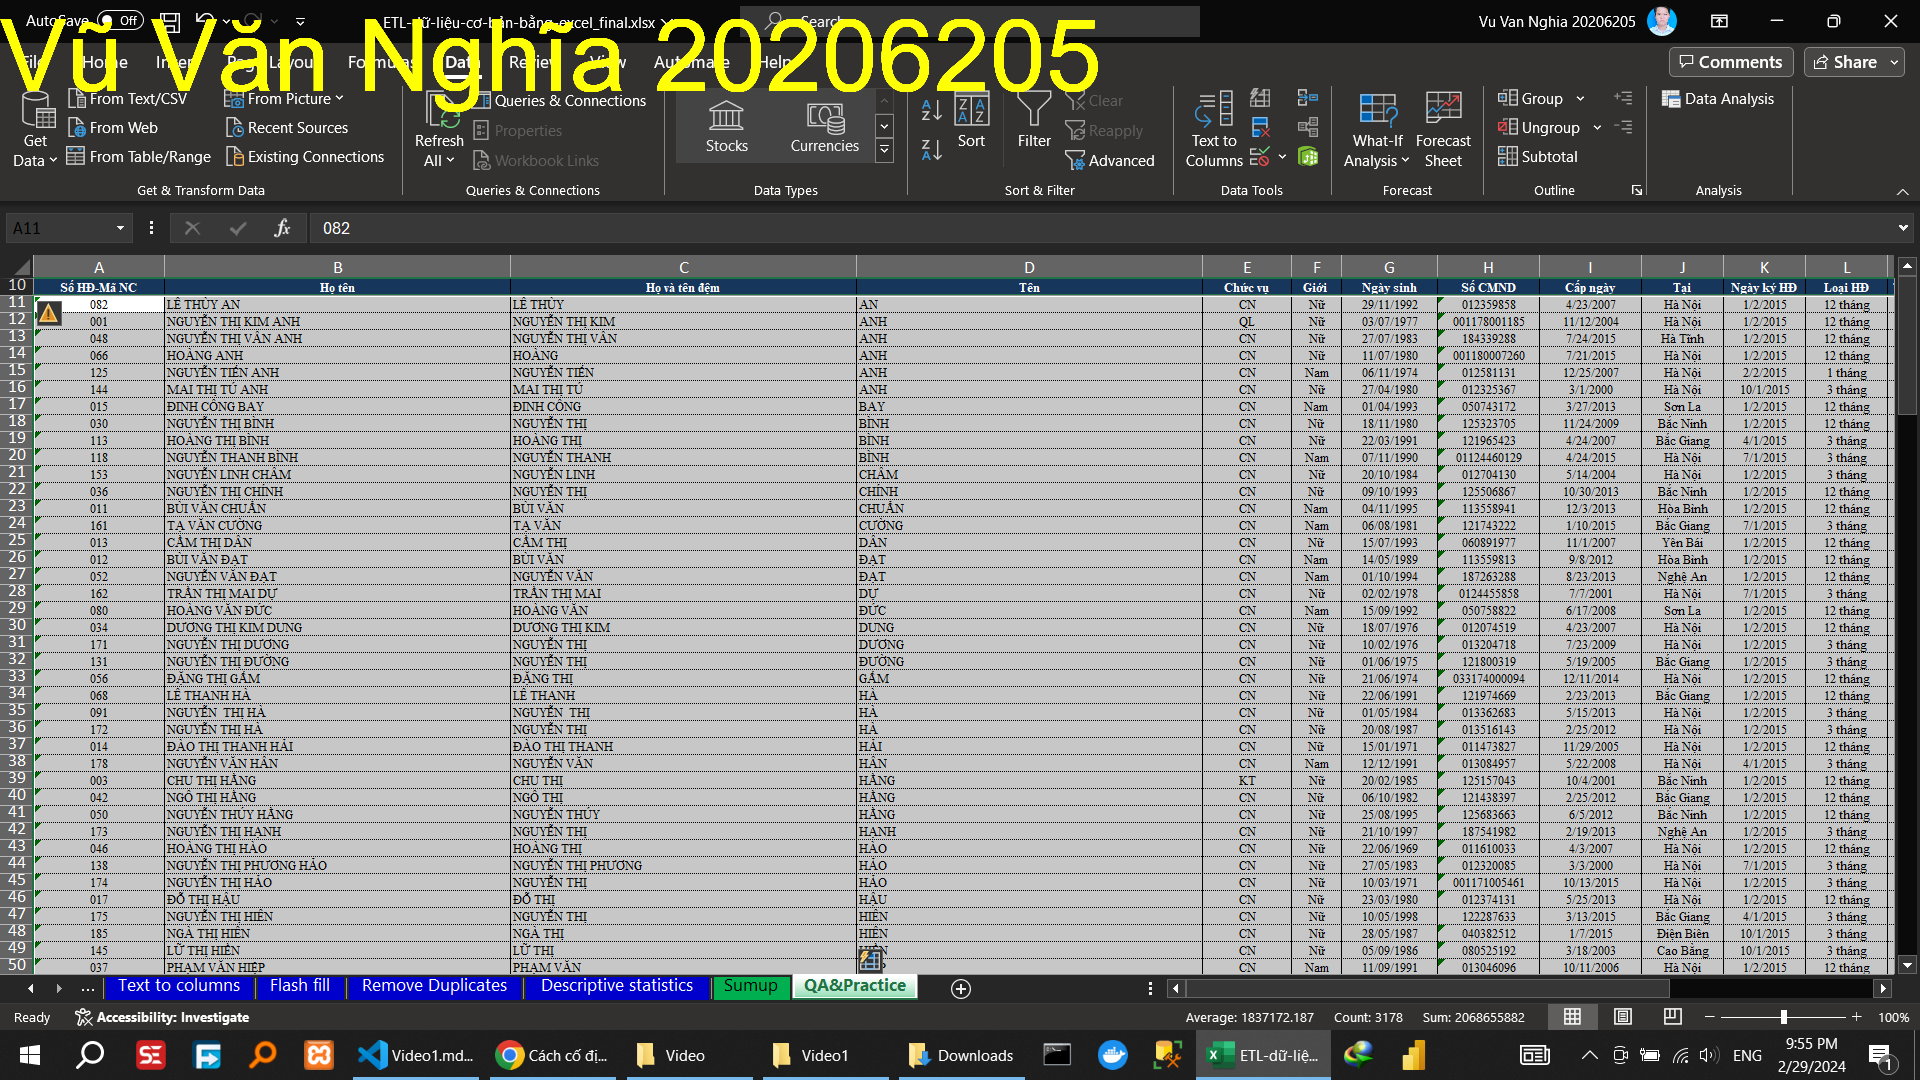
\includegraphics[scale = 0.15]{Video1/ThucHanh/5.png}
\caption{Thực hành  sắp xếp danh sách theo tên nhân công}
\end{figure}

% <!-- Lập danh các chức vụ của mỗi bộ phận ( Remove Duplicates) -->


% \paragraph{Thực hành  lập danh  sách các chức vụ của mỗi bộ phận}
% \subparagraph{Thực hành  lập danh  sách các chức vụ của mỗi bộ phận}
\begin{figure}[h]
    \centering
    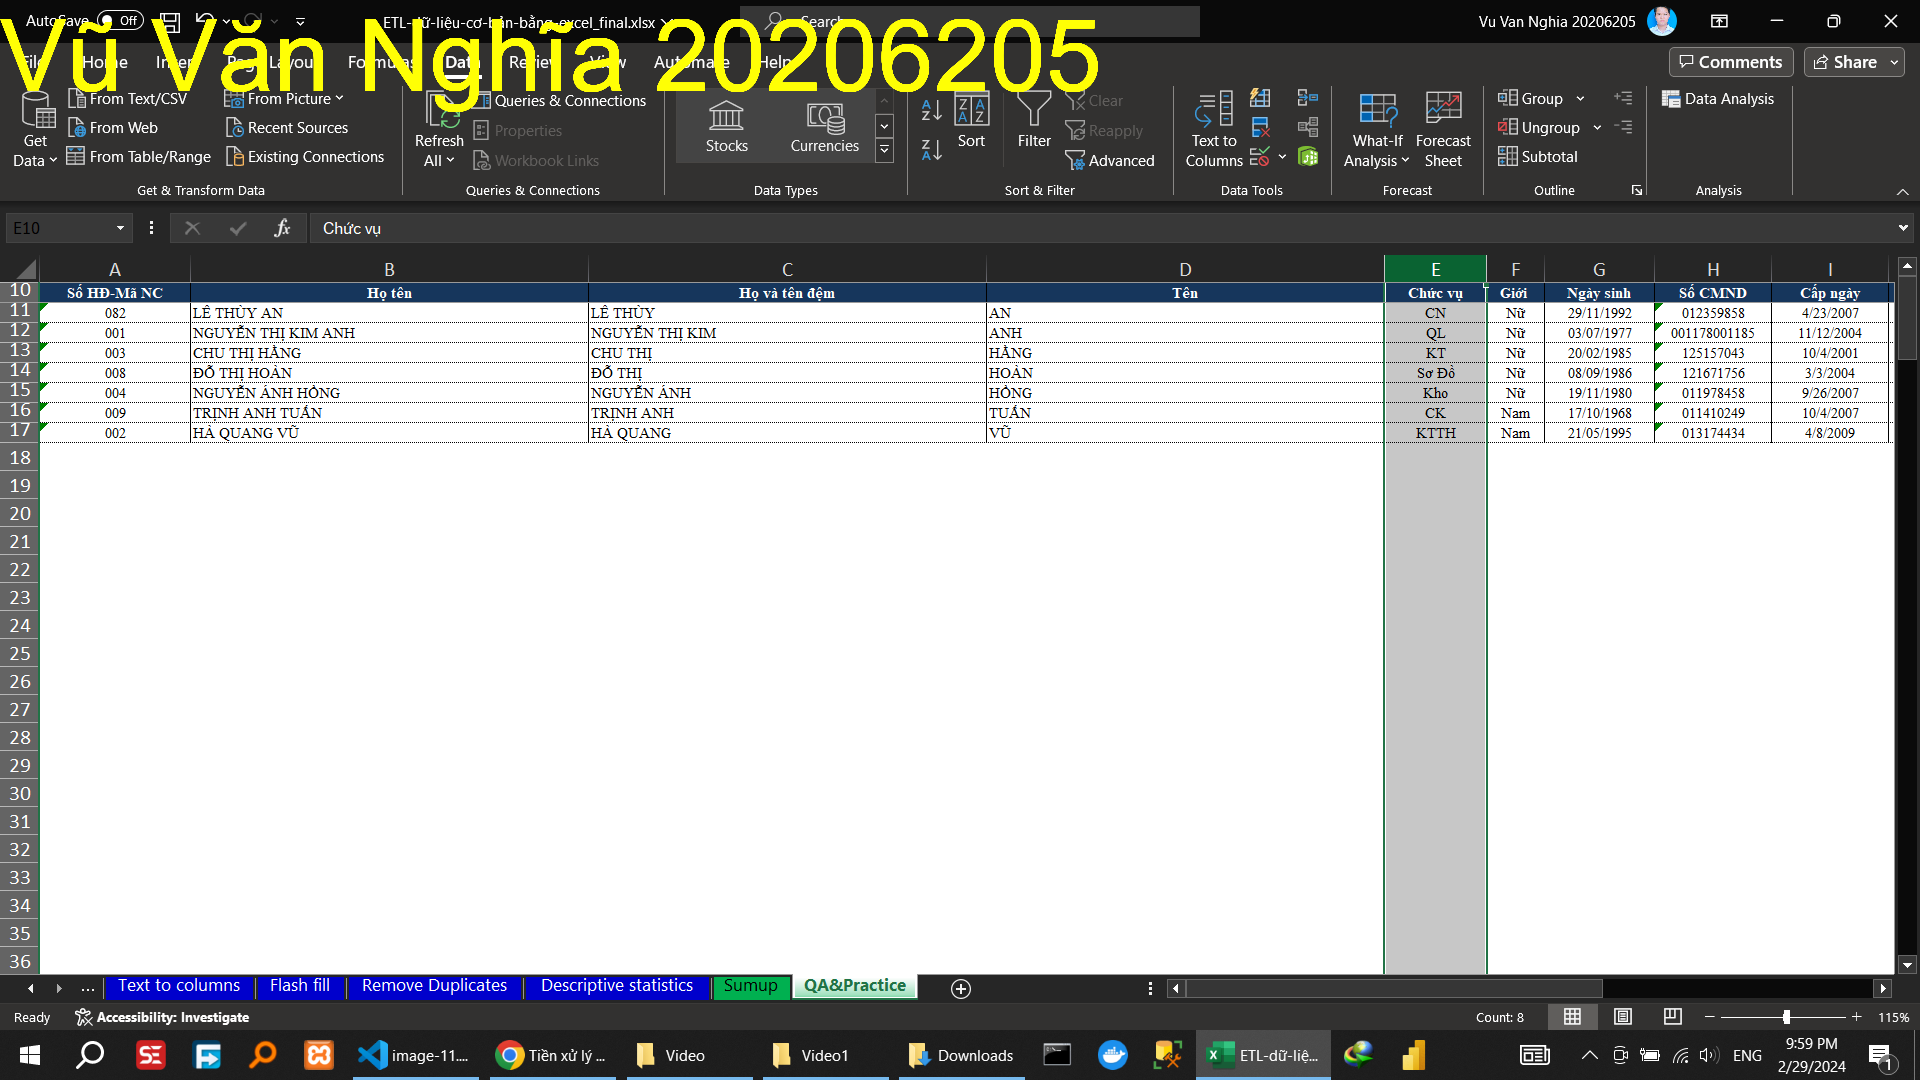
\includegraphics[scale = 0.15]{Video1/ThucHanh/6.png}
\caption{Thực hành  lập danh  sách các chức vụ của mỗi bộ phận}
\end{figure}



\subsection{Video 2}
\subsubsection{Hướng dẫn}

\subsubsection{Thực hành}




\subsection{Video 3}
\subsubsection{Hướng dẫn}

\subsubsection{Thực hành}




\subsection{Video 4}
\subsubsection{Hướng dẫn}

\subsubsection{Thực hành}




\subsection{Video 5}
\subsubsection{Hướng dẫn}

\subsubsection{Thực hành}




\subsection{Video 6}
\subsubsection{Hướng dẫn}

\subsubsection{Thực hành}




\subsection{Video 7}
\subsubsection{Hướng dẫn}

\subsubsection{Thực hành}




\subsection{Video 8}
\subsubsection{Hướng dẫn}

\subsubsection{Thực hành}








%%%%%%%%%%%%%%%%%%%%%%%%%%%%%%%%%%%%%%%%%%%%%%%%%%%%%%%
\end{document}
%%%%%%%%%%%%%%%%%%%%%%%%%%%%%%%%%%%%%%%%%%%%%%%%%%%%%%%





\begin{figure}[h]
    \centering
    \includegraphics[width=0.5\textwidth]{example-image-a}
    \caption{Ví dụ về hình ảnh}
    \label{fig:example}
\end{figure}